\documentclass[12pt, a4paper, twoside]{book}
\usepackage[utf8]{inputenc}
\usepackage[english, serbianc]{babel}
\usepackage{lipsum}
\usepackage{graphicx}
\usepackage{xcolor}
\usepackage{multicol}
\usepackage{booktabs}
\usepackage{nicefrac}
\usepackage{subcaption}
\usepackage{float}
\usepackage{tikz}
\usetikzlibrary{calc}
\usetikzlibrary{calc, arrows.meta, positioning, backgrounds}
\usetikzlibrary{perspective}

\usepackage{geometry}
\geometry{
	a4paper,
	total={160mm,237mm},
	left=30mm,
	top=30mm,
}

\usepackage{hyperref}
\usepackage{xcolor}
\hypersetup{
	colorlinks,
	linkcolor={red!50!black},
	citecolor={blue!50!black},
	urlcolor={blue!80!black}
}

\usepackage{fancyhdr}
\pagestyle{fancy}
\fancyhead{}
\fancyhead[RE]{\leftmark}
\fancyhead[LO]{\rightmark}
\fancyfoot{}
\fancyhead[LE, RO]{\thepage}

\usepackage{amsmath}
\usepackage{bm}
\usepackage{amsthm}
\usepackage{amssymb}
\numberwithin{equation}{chapter}
\newtheorem{theorem}{Теорема}
\numberwithin{theorem}{section}
\newtheorem{definition}{Дефиниција}
\numberwithin{definition}{section}
\newtheorem{definitionChapter}{Дефиниција}
\numberwithin{definitionChapter}{chapter}

\begin{document}	
\begin{titlepage}
	\newcommand{\HRule}{\rule{\linewidth}{0.5mm}}
	\center
	
	\textbf{\LARGE УНИВЕРЗИТЕТ У БЕОГРАДУ\\MАТЕМАТИЧКИ ФАКУЛТЕТ}
	\begin{figure}[!ht]
		\centering
		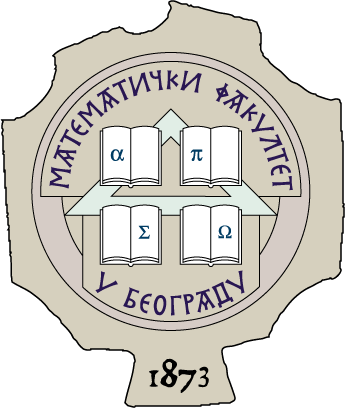
\includegraphics[width=0.2\textwidth]{img/matf-logo.png}
	\end{figure}\\[3cm]
	\textbf{\Large МАСТЕР РАД}\\[0.3cm]
	на катедри за \\[0.3cm]
	\textbf{\Large Рачунарство и информатику}\\[.7cm] % Minor heading such as course title
	на тему\\[0.7cm]
	
	\HRule \\[0.4cm]
	{ \huge \bfseries Примена неуронских поља зрачења у рендеровању}\\[0.4cm] % Title of your document
	\HRule \\[1.5cm]
	
	\begin{minipage}{0.4\textwidth}
		\begin{center}
			Коста Грујчић
		\end{center}
	\end{minipage}\\[5cm]
	
	{\large Београд, \today}\\[2.5cm]
	\vfill
\end{titlepage}
\pagenumbering{roman}

% Defines mentor & date
\newpage
\thispagestyle{empty}

\hspace{0pt}
\vfill
\noindent \textbf{Ментор}:\\
проф. др Младен Николић\\Универзитет у Београду, Математички факултет
\\[2cm]

\noindent \textbf{Чланови комисије}:
\\проф. др Младен Николић\\Универзитет у Београду, Математички факултет
\\[0.25cm]
\\проф. др Младен Николић\\Универзитет у Београду, Математички факултет
\\[0.25cm]
\\проф. др Младен Николић\\Универзитет у Београду, Математички факултет
\\[2cm]

\noindent \textbf{Датум одбране}: \today
\hspace{0pt}
\vfill

\newpage
\thispagestyle{empty}
\textit{Својој мајци}

\newpage
\thispagestyle{empty}
\noindent \textbf{Наслов мастер рада}: Примена неуронских поља зрачења у рендеровању

\noindent \textbf{Резиме}:

\noindent \textbf{Кључне речи}: машинско учење, неуронска поља, рендеровање

\listoffigures
\listoftables
\tableofcontents

\pagenumbering{arabic}
\chapter{Увод}
Рендеровање је проблем стар колико и рачунарска графика. Постоји небројано пуно различитих
алгоритама, приступа, техника и хеуристика за решавање овог важног проблема, а управо је
рендеровање покретач низа хардверских унапређења у деценијама иза нас. С друге стране,
машинско учење и вештачка интелигенција уопште, су изузетно актуелна област истраживања и примене.
Употреба машинског учења у домену рачунарског вида је довела до неслућених успеха и унапређења
чак и у свакодневном животу. Тако се природно дошло до \textit{неуронског рендеровања},
односно, рендеровања сцене употребом неуронских мрежа које су засигурно најпознатија фамилија модела
машинског учења.

Неуронска поља зрачења су један од водећих новитета машинског учења, нарочито у оквиру
подобласти рачунарског вида. У питању су врсте неуронских мрежа посебно намење за учење векторских поља.
Будући да је рендеровање центар интересовања, реч је о специфичној врсти поља којима се описује боја
сваке тачке. Имају широку, пре свега, генеративну примену и представљају изузетно живу научну тему.
Отуда се и јавила идеја темељног заснивања ове врсте модела као и њиховог упоређивања на основу добијених
резултата.

Како је у рачунарству од велике важности и пратећа имплементација, значај овог рада можемо видети 
и у чињеници да су сви модели у потпуности имплементирани. То за последицу има једноставан поступак
обучавања као и употребе.

Један од споредних циљева овог рада је превођење израза који су се безразложно одомаћили
у српској научној заједници као англицизми. С друге стране, скраћенице остају у изворном
облику и то на латиници, што читаоцу пружа могућност за непосредно претраживање навода.

Битно је напоменути да слике овог рада нису ауторске, већ су преузете из одговарјаућих научних радова
који су јавно доступни. Њихов изворни облик је задржан, уз превођење појединих делова уколико је за
тим било потребе.

\chapter{Основни појмови рачунарске графике}
\section{Светлост и боја}
Светлост представља електромагнетно зрачење чија је таласна дужина у сегменту од око 350 до
700 nm, које побуђује визуелни систем човека. То значи да људи \textit{не виде} светлост
осталих таласних дужина, тако да ћемо убудуће под видљивим спектром светлости мислити управо
на овај, видљив човеку.

%Светлост коју наш визуелни систем региструје мора доћи од неког извора. Тако и разликујемо
%примарне и секундарне изворе светлости, односно изворе који производе зрачење и оне који их
%само рефлектују. Када је реч о рефлексији светлости, она може бити спекуларна када се светлост
%рефлектује дуж тачно једног правца, или дифузна када се расипа.

Потребно је увести физичке величине којима се могу квантификовати основна физичка својства
светлости. Прво ћемо дефинисати радиометријске величине, а онда одговарајуће фотометријске.

\begin{definition}
	Фотон је квант електромагнетног зрачења. Енергија фотона је:
	$$E=\frac{hc}{\lambda} \left[\mathrm{J}\right],$$ где је $h$ Планкова константа, $c$ брзина светлотси, а $\lambda$ 
	таласна дужина фотона.
\end{definition}

\begin{definition}
	Укупна енергија зрачења извора зрачења је: $$Q_e = \int_{S^2} E d\Omega \left[\mathrm{J}\right].$$
\end{definition}

\begin{definition}
	Флукс зрачења је укупна енергија зрачења која доспе на неку површину по јединици времена:
	$$\Phi_e = \frac{\partial Q_e}{\partial t} \left[\mathrm{W}\right].$$
\end{definition}

\begin{definition}
	Озраченост је укупан флукс зрачења по јединици површине:
	$$E_e = \frac{\partial \Phi_e}{\partial A} \left[\mathrm{\frac{W}{m^2}}\right].$$
\end{definition}

\begin{definition}
	Јачина зрачења је укупан флукс зрачења у неком смеру по јединичном просторном углу:
	$$I_{e, \Omega} = \frac{\partial \Phi_e}{\partial \Omega} \left[\mathrm{\frac{W}{sr}}\right].$$
\end{definition}

\begin{definition}
	Зрачење је је укупан флукс зрачења у неком смеру по јединици површине и јединичном просторном углу:
	$$L_{e, \Omega} = \frac{\partial^2 \Phi_e}{\partial \Omega \partial A} \left[\mathrm{\frac{W}{sr \cdot m^2}}\right].$$
\end{definition}

Спектралне величине се дефинишу у односу на таласну дужину. На пример, спектрално зрачење
је $L_{e, \Omega, \lambda} = \nicefrac{\partial L_{e, \Omega}}{\partial \lambda}$.
Аналогно и за остале.

Након дефинисања мноштва физичких величина, коначно долазимо и до фотометријских, или како се
још називају и \textit{визуелне}. Кључна разлика у односу на радиометријске, или како се још
називају и \textit{енергетске}, је што се у овом случају у обзир узима и спектрална
осетљивост посматрача. То одговара интуитивном поимању светлости -- човек светлост разликује на
основу боје, што је у директној коресподенцији са таласном дужином.

У основи спектралне зависности посматрача је \textbf{\textit{функција релативне светлосне осетљивости}} $V$.
Помоћу ове функције изражавамо просечну осетљивост човека на светлост одређене таласне дужине.
Просечна је у смислу да може варирати у популацији, али представља врло добру апроксимацију
у општем случају, поготово имајући у виду да је стандардизована од стране Међународног комитета
за осветљење.

\begin{definition}
	Светлосни флукс је укупна енергија која протекне кроз неку површину у јединици времена:
	$$\Phi_v = K\int_{0}^{\infty}\Phi_{e, \lambda} V(\lambda)d\lambda \left[\mathrm{lm}\right].$$
	\label{eqn-luminuous-flux}
\end{definition}

За вредност онстанте $K$ из \ref{eqn-luminuous-flux} се узима $683.002 \mathrm{\frac{lm}{W}}$. Реч
је о још једној примеру стандардизације у области фотометрије.

\begin{definition}
	Јачина светлости је укупна снага коју емитује извор светлости у одређеном смеру по јединичном
	просторном углу:
	$$I_v = K \int_{0}^{\infty}I_{e, \lambda}V(\lambda)d\lambda \left[\mathrm{cd}\right].$$
\end{definition}

\begin{definition}
	Осветљеност је укупан светлосни флукс на некој површини:
	$$E_v = K\int_{0}^{\infty}I_{e, \lambda}E_{e, \lambda}V(\lambda)d\lambda \left[\mathrm{lx}\right].$$
\end{definition}

\begin{definition}
	Сјајност је укупан светлоснi флукс који напушта, пролази или пада на површину по јединичном просторном
	углу и по ортогоналној пројекцији јединичне површине:
	$$L_v = \frac{\partial^2\Phi_v}{\partial\Omega\partial A \cos\theta} \left[\mathrm{\frac{cd}{m^2}}\right].$$
\end{definition}

Сјајност је једина фотометријска величина коју човек непосредно опажа. Она представља мерило за субјективни утисак
о мањој или већој сјајности светлеће или осветљене површине.

Већ смо поменули да људи разликују неке таласне дужине светлости, односно виде светлост одређене боје. Ту
способност нам дају три врсте чепића који се налазе у жутој мрљи мрежњаче ока. Према томе, кроз ове рецепторе,
наш мозак прима свега три врсте сигнала за сваки очни надражај. Међутим, људско око није идеалан спектрометар, па
поједине таласе просто види као светлост исте боје.

Зато се боја на рачунару представља тројкама $(R, G, B)$ где су координате удео црвене, плаве и зелене боје редом, које
се узимају за основне. Постоје и други системи боја попут HSV или CMYK, али о њима неће бити речи јер ћемо надаље
користити искључиво RGB систем.

На овај начин је могуће чувати тачно $255^3$ боја, што је и више него довољно будући да људско око разликује до 10
милиона боја. Даља практична ограничења се тичу квалитета монитора као и графичког процесора, али се тиме нећемо бавити.

%Фотометријске величине су аналогони радиометријских и даћемо их у поређењу са
%радиометријским величинама табелом \ref{table-radio-vs-photo}.

%\begin{table}[h]
%	\centering
%	\begin{tabular}{|l|l|}
%		\hline
%		{\textbf{Радиометријске величине}} & {\textbf{Фотометријске величине}}\\
%		\hline
%		{Флукс зрачења $\left[W\right]$} & {Светлосни флукс $\left[lm\right]$} \\ 
%		\hline
%		{Озраченост $\left[\frac{W}{m^2}\right]$} & {Осветљеност $\left[lx\right]$} \\
%		\hline
%		{Јачина зрачења $	\left[\frac{W}{sr}\right]$} & {Јачина светлости $\left[cd\right]$} \\
%		\hline
%		{Зрачење $\left[\frac{W}{sr \cdot m^2}\right]$} & {Сјајност $\left[\frac{cd}{m^2}\right]$}\\
%		\hline
%	\end{tabular}
%	\caption{Поређење радиометријских и фотометријских величина}
%	\label{table-radio-vs-photo}
%\end{table}

\section{Камера}
Можемо сматрати да нам је појам камере познат из стварног света. У овој глави
ћемо строго дефинисати камеру и дати један од многобројних начина њеног
моделовања у домену рачунарске графике.

\begin{definition}
	Камера је пресликавање из $\mathbb{R}^3$ у $\mathbb{R}^2$.
\end{definition}

У питању је врло општа, готово бескорисна дефиниција. Међутим, ако размислимо
о томе да се стваран свет врло добро може представити као простор димензије $3$,
а да се фотографија може схватити као раван, можемо увидети да је у питању заиста
исправна формулација. Оно што овом дефиницијом није обухваћено јесте како се тачно
од света око нас долази до слике. Зато има смисла говорити о моделима камере као
различитим парадигмама изведбе поменутог пресликавања. У овом раду ће највише
бити коришћен тачкасти модел камере тако да ћемо у наставку поглавља дати његову
прецизну дефиницију.
	
	\subsection{Тачкасти модел камере}
	Посматрајмо канонски Еуклидски простор димензије $3$ и раван $z=f$ коју ћемо звати
	\textbf{\textit{раван слике}}. У овом моделу камере се произвољна тачка $\mathbf{x_w}=(x, y, z)$ из простора
	пресликава у тачку $\mathbf{x_p}=(u,v)$ која је тачка пресека равни слике и праве која спаја $\mathbf{x_w}$
	и центар камере $\mathbf{c}$, који ћемо за сад поставити у координатни почетак.	Другим речима, у питању је централна
	пројекција са центром у координатном почетку. Тривијалном применом сличности троуглова долазимо до
	
	\begin{equation}
		(x, y, z) \mapsto (\nicefrac{fx}{z}, \nicefrac{fy}{z}).
	\end{equation}

	Права која пролази кроз центар камере и нормална је на раван слике називамо \textbf{\textit{главном осом}},
	а тачка у којој се главна оса и раван слике секу називамо \textbf{\textit{главном тачком}}.
	
	Приметимо још једну особину централног пројектовања -- све тачке праве која пролази кроз центар
	камере се пројектују у исту тачку равни слике. Зато ћемо увести хомогене координате. Отуда
	можемо писати $\mathbf{x_p} = P\mathbf{x_w}$. Овакво пресликавање се може преписати и у
	матричном облику
	
	\begin{equation}
		\begin{bmatrix}
			x \\
			y \\
			z \\
			1
		\end{bmatrix}
		\mapsto
		\begin{bmatrix}
			fx \\
			fy \\
			z
		\end{bmatrix}
		=
		\begin{bmatrix}
			f && 0 && 0 && 0 \\
			0 && f && 0 && 0 \\
			0 && 0 && 1 && 0
		\end{bmatrix}
		\begin{bmatrix}
			x \\
			y \\
			z \\
			1
		\end{bmatrix}.
		\label{eqn-px}
	\end{equation}

	Ради конзистентности са наставком, раставићемо $P$ на прозивод
	\begin{equation}
		K
		\begin{bmatrix}
			R && t
		\end{bmatrix},
		\label{eqn-krt}
	\end{equation}
	где je $K \in M_{3, 4}(\mathbb{R})$, $R \in M_{3, 3}(\mathbb{R})$ и $t \in M_{3, 1}(\mathbb{R})$.
	Уклањајући последњу колону из \ref{eqn-px} добијамо матрицу $K$ из овако измењеног пресликавања.
	
	Уколико уопштимо положај главне тачке и њене координате означимо са $(p_x, p_y)$, матрица $K$
	поприма облик
	
	\begin{equation}
		\begin{bmatrix}
			f && 0 && p_x \\
			0 && f && p_y \\
			0 && 0 && 1
		\end{bmatrix}.
	\end{equation}

	Коначно, можемо уопштити и положај центра камере. Тада уочавамо два координатна система -
	онај с почетка, канонски, у ком нам је лако да баратамо и други, са центром камере као
	координатним почетком. Није тешко увидети да се кретањем (ротацијом и транслацијом) репер камере
	може довести до канонског. На тај начин употпуњујемо пресликавање $P$. На слици \ref{fig-pinhole} 
	је дата интепретација овог пресликавања.
	
	\begin{figure}[H]
		\begin{center}
		\begin{tikzpicture}
			% Picture's vectors definition
			\def\xOne{1}
			\def\xTwo{0.5}
			\def\yOne{0}
			\def\yTwo{-1.3}
			\def\zOne{-1}
			\def\zTwo{0.5}
			
			% CAMERA COORDINATE SYSTEM
			%\draw[thick,->] (0,0) -- (\xOne,\xTwo) node[anchor=north]{$x$};
			%\draw[thick,->] (0,0) -- (\yOne,\yTwo) node[anchor=west]{$y$};
			%\draw[thick,->] (0,0) -- (\zOne,\zTwo) node[anchor=north,yshift=-2pt,xshift=3pt]{$z$};
			\draw[very thick,->] (-\zOne/2,-\zTwo/2) -- (-\zOne/2+\xOne,-\zTwo/2+\xTwo) node[anchor=north west, xshift=-3pt,font=\footnotesize]{$\mathbf{e_x}$};
			\draw[very thick,->] (-\zOne/2,-\zTwo/2) -- (-\zOne/2+\yOne,-\zTwo/2+\yTwo) node[anchor=west,font=\footnotesize]{$\mathbf{e_y}$};
			\draw[very thick,->] (-\zOne/2,-\zTwo/2) -- (\zOne/2,\zTwo/2) node[anchor=north,yshift=-2pt,xshift=3pt,font=\footnotesize]{$\mathbf{e_z}$};
			\draw (-\zOne/2,-\zTwo/2) node[anchor=north west,font=\footnotesize]{$\mathbf{c}$};
			
			% CAMERA AXIS ELONGATION
			\draw[very thin,solid] (-\zOne/2-2*\xOne,-\zTwo/2-2*\xTwo) -- (-\zOne/2+2*\xOne,-\zTwo/2+2*\xTwo); % x elongation
			\draw[very thin,solid] (3*\zOne,3*\zTwo) -- (6*\zOne,6*\zTwo); % optical axis behind projection plane
			
			% REFERENCE LINES
			%\draw[thin,dashed] (1.4*\xOne-\zOne/2,1.4*\xTwo-\zTwo/2) -- (6*\zOne+1.4*\xOne,6*\zTwo+1.4*\xTwo); % object x position
			\draw[very thin,solid] (6*\zOne-2*\xOne,6*\zTwo-2*\xTwo) -- (6*\zOne+2*\xOne,6*\zTwo+2*\xTwo) node[anchor=west]{}; %object z position
			
			% WORLD OBJECT
			\draw[line width=1pt,blue,line cap=round] (6*\zOne+1.4*\xOne,6*\zTwo+1.4*\xTwo) -- (6*\zOne+1.4*\xOne,6*\zTwo+1.4*\xTwo+1.1) node[anchor=south,font=\footnotesize]{$\mathbf{x}_w=(x,y,z)$};
			\node[circle,inner sep=0pt,minimum size=0.2cm,fill=blue] (object) at (6*\zOne+1.4*\xOne,6*\zTwo+1.4*\xTwo+1.1) {};
			
			% PROJECTION LINE BEHIND PROJECTION PLANE
			\draw[thick,solid,red] (3*\zOne+0.69*\xOne,3*\zTwo+0.7*\xTwo+0.69) -- (6*\zOne+1.4*\xOne,6*\zTwo+1.4*\xTwo+1.1);
			
			%% PROJECTION PLANE
			\filldraw[fill=gray!20,draw=gray!70,opacity=0.8] (3*\zOne-1.5*\xOne-1.5*\yOne,3*\zTwo-1.5*\xTwo-1.5*\yTwo) -- (3*\zOne+1.5*\xOne-1.5*\yOne,3*\zTwo+1.5*\xTwo-1.5*\yTwo) -- (3*\zOne+1.5*\xOne+1.5*\yOne,3*\zTwo+1.5*\xTwo+1.5*\yTwo) -- (3*\zOne-1.5*\xOne+1.5*\yOne,3*\zTwo-1.5*\xTwo+1.5*\yTwo) -- (3*\zOne-1.5*\xOne-1.5*\yOne,3*\zTwo-1.5*\xTwo-1.5*\yTwo);
			
			% PLOJECTION PLANE COORDINATE SYSTEM u,v
			\draw[->,thick,green!70!black,dashed] (3*\zOne-1.5*\xOne-1.5*\yOne,3*\zTwo-1.5*\xTwo-1.5*\yTwo) -- (3*\zOne+2*\xOne-1.5*\yOne,3*\zTwo+2*\xTwo-1.5*\yTwo)
			node[anchor=north west, xshift=-3pt,font=\footnotesize]{$u$};
			\draw[->,thick,green!70!black,dashed] (3*\zOne-1.5*\xOne-1.5*\yOne,3*\zTwo-1.5*\xTwo-1.5*\yTwo) -- (3*\zOne-1.5*\xOne-1.5*\yOne,3*\zTwo-1.5*\xTwo+2*\yTwo)
			node[anchor=west,font=\footnotesize]{$v$};
			
			% PROJECTION PLANE COORDINATE SYSTEM x,y
			\draw[->,thick,gray,dashed] (3*\zOne-2*\xOne,3*\zTwo-2*\xTwo) -- (3*\zOne+2*\xOne,3*\zTwo+2*\xTwo)
			node[anchor=north west, xshift=-3pt,font=\footnotesize]{$x$};
			\draw[->,thick,gray,dashed] (3*\zOne-2*\yOne,3*\zTwo-2*\yTwo) -- (3*\zOne+2*\yOne,3*\zTwo+2*\yTwo)
			node[anchor=west,font=\footnotesize]{$y$};
			
			% PROJECTION  OBJECT
			\draw[line width=1pt,blue,line cap=round] (3*\zOne+0.69*\xOne,3*\zTwo+0.69*\xTwo) -- (3*\zOne+0.69*\xOne,3*\zTwo+0.69*\xTwo+0.69);
			\node[circle,inner sep=0pt,minimum size=0.1cm,fill=blue] (object) at (3*\zOne+0.69*\xOne,3*\zTwo+0.7*\xTwo+0.69) {};
			
			% PIXEL OBJECT
			\filldraw[red,opacity=0.6] (3*\zOne+6*0.105*\xOne,3*\zTwo+0.75+6*0.105*\xTwo) -- ++(0.105*\xOne,0.105*\xTwo) -- ++(0.105*\yOne,0.105*\yTwo) -- ++(-0.105*\xOne,-0.105*\xTwo) -- ++(-0.105*\yOne,-0.105*\yTwo);
			
			% PROJECTION LINE IN FRONT OF PROJECTION PLANE
			\draw[thick,solid,red] (-\zOne/2,-\zTwo/2) -- (3*\zOne+0.69*\xOne,3*\zTwo+0.7*\xTwo+0.69);
			
			% OPTICAL AXIS IN FRONT OF PROJECTION PLANE
			\draw[thin,solid] (0,0) -- (3*\zOne,3*\zTwo);
			
			% ANNOTATIONS
			% z = f
			\draw (3*\zOne-1*\xOne+1.3*\yOne,3*\zTwo-1*\xTwo+1.3*\yTwo) node[gray!70,rotate=28,font=\scriptsize] {$z=f$};
			%		% bar(u)
			%		\draw[to-to, green!70!black] (3*\zOne+0.13*\xOne+0.08*\yOne,3*\zTwo+0.13*\xTwo+0.08*\yTwo) -- (3*\zOne+0.7*\xOne+0.08*\yOne,3*\zTwo+0.7*\xTwo+0.08*\yTwo) node[midway,anchor=north west,xshift=-2pt,yshift=2pt,font=\scriptsize] {$ \bar{u} $};
			%		% bar(v)
			%		\draw[to-to, green!70!black] (3*\zOne-0.1*\xOne-0.04*\yOne,3*\zTwo-0.1*\xTwo-0.04*\yTwo) -- (3*\zOne-0.1*\xOne,3*\zTwo-0.1*\xTwo+0.75) node[midway,anchor=east,xshift=2pt,font=\scriptsize] {$ \bar{v} $};
			% (u,v)
			\node[green!70!black,anchor=west,font=\scriptsize] at (3*\zOne+0.69*\xOne-0.1,3*\zTwo+0.7*\xTwo+0.89) {$\mathbf{x_p}=(u,v)$};
			% principal point
			\draw[very thin] (3*\zOne-0.02*\xOne+0.02*\yOne,3*\zTwo-0.02*\xTwo+0.02*\yTwo) .. controls (3*\zOne-0.1*\xOne+0.3*\yOne,3*\zTwo-0.1*\xTwo+0.3*\yTwo) and (3*\zOne-0.3*\xOne+0.1*\yOne,3*\zTwo-0.3*\xTwo+0.1*\yTwo) ..  (3*\zOne-0.6*\xOne+0.4*\yOne,3*\zTwo-0.6*\xTwo+0.4*\yTwo) node[anchor=north,align=center,font=\scriptsize] {главна тачка};
			
			% optical axis
			\draw[very thin] (5.5*\zOne-0.02*\xOne+0.02*\yOne,5.5*\zTwo-0.02*\xOne+0.02*\yOne) .. controls (5.5*\zOne-0.1*\xOne+0.3*\yOne,5.5*\zTwo-0.1*\xTwo+0.3*\yTwo) and (5.5*\zOne-0.3*\xOne+0.1*\yOne,5.5*\zTwo-0.3*\xTwo+0.1*\yTwo) ..  (5.5*\zOne-0.6*\xOne+0.4*\yOne,5.5*\zTwo-0.6*\xTwo+0.4*\yTwo) node[anchor=north,align=center,font=\scriptsize] {главна оса};
		\end{tikzpicture}
		\end{center}
		\caption{Интерпретација тачкастог модела камере}
		\label{fig-pinhole}
	\end{figure}
	
	Постоји укупно $9$ слободних параметара -- по $3$ за сваку од матрица $K$, $R$ и $t$.
	Матрица $K$ се назива \textbf{\textit{матрица калибрације}}, а њене вредности \textbf{\textit{унутрашњим параметрима}}
	камере. Вредности матрице $\begin{bmatrix}R && t\end{bmatrix}$ се називају \textbf{\textit{спољашњим параметрима}}
	камере.
	
	Поменимо још једну терминолошку конвенцију. Координатни систем из којег вршимо пројекцију се 
	назива и \textbf{\textit{светским координатним системом}}, а координатни систем индукован положајем
	камере \textbf{\textit{координатни систем камере}}. \textbf{\textit{Координатни систем слике}} је
	онај везан за раван слике.

	Корисно је дати додатни коментар у вези са нулом у првом реду матрице калибрације. У питању је коецифијент
	смицања којим је могуће уопштити раван слике -- правоугаоник постаје паралелограм.

\section{Рендеровање}
Када смо говорили о камери, видели смо да слика није ништа друго до дводимензиона пројекција стварног света.
Слично је и када комплексну сцену, овог пута виртуелног, света желимо да прикажемо на монитору. Мора доћи
до пројектовања света, а слику коју видимо је уствари слика добијена посматрањем света кроз виртуелну камеру.
Тај процес се назива \textbf{\textit{рендеровање}}. Дакле, рендеровањем се од сцене долази до конкретне
репрезентације слике у пикселима.

Пре него што се упустимо у рендеровање, вратимо се корак уназад. Светлост и камеру смо, на први поглед, увели
врло неповезано. Светлост смо дефинисали више експериментално ослањајући се на физичке законе, док смо камеру
увели строго геометријски. Сада ћемо оба појма ставити у контекст и објаснити њихову везу.

Праве које смо уочавали у моделу камере су светлосни зраци. Раван слике у пракси није бесконачна, већ има своју
ширину и дужину којима се одређују димензије слике. Такође, услед физичких ограничења слика се мора дискретизовати.
Посматрамо ли слику на тај начин, видећемо да је она матрица чије елементе називамо \textbf{\textit{пикселима}}.
Како ће који пиксел да изгледа, oдносно које ће боје бити, одређује количина зрачења која допре до камере.
Зрачење смо увели у зависности од правца, што у комбинацији са пројективним особинама модела камере одређује
који ће пиксел \textit{бити погођен}. Такође, природно је увести ограничење по питању дела простора који
камера може да опажа. Величину слике смо већ поменули, али не и параметар по $z$ оси. Ради једноставности
геометрије, уводимо \textbf{\textit{предњу и задњу раван одсецања}}. Све испред предње и иза задње равни одсецања
не утиче на резултујућу слику.

\subsection{Запреминско рендеровање}
Посматрајмо шта се дешава са светлости приликом проласка кроз неку средину. Може доћи до:
\begin{itemize}
	\item упијања -- средина упија фотоне светлосног зрака приликом чега се ослобађа топлота
	или неки други вид енерије.
	\item емисије -- како је светлост зрачење, пролазак светла кроз средину је загрева.
	Када средина достигне одрђену температуру, може доћи до емитовања светлости.
	\item расипања -- део фотона напушта правац зрака што доводи до мешања фотона
	са различитих праваца.
\end{itemize}

Према томе, више чинилаца утиче на коначно зрачење које ће путем неког светлосног зрака доћи до камере.
Тачке неког светлосног зрака с почетком у $\mathbf{o}$ и правцем $\mathbf{d}$ једнозначно одређујемо
као $\mathbf{r_{o, d}}(t) = \mathbf{o} + t\mathbf{d}$.

Нека су предња и задња раван одсецања редом $z=t_n$ и $z=t_f$, а светлосне зраке посматрамо из положаја
камере $\mathbf{c}$. Према томе, до камере дуж зрака $\mathbf{r_{c, d}}$ допире следећа
количина зрачења

\begin{equation}
	\int_{t_n}^{t_f}T(t)\sigma(\mathbf{r_{c, d}}(t))L_{e, \Omega}\bigr|_{\mathbf{r_{c, d}}(t)}dt,
	\label{eqn-volume-rendering-radiance}
\end{equation}

где је $T(t)=\exp{\left(-\int_{t_n}^{t}\sigma(\mathbf{r_{c, d}}(s)ds)\right)}$ акумулирана пропусност
зрака од $t_n$ до $t$. Ова величина представља вероватноћу да светлосни зрак на путу од $t_n$ до
$t$ не удари нити у једну препреку. Напоменимо да се интеграција врши искључиво по фотонима
који се налазе на светлосном зраку од интереса, или другим речима, интеграли се само по
расутој светлости.

Како нам је боја пиксела крајњи циљ, једначину \ref{eqn-volume-rendering-radiance} ћемо
преписати у колориметријском облику

\begin{equation}
	C(\Pi_{\mathbf{r_{c, d}}}) = \int_{t_n}^{t_f}T(t)\sigma(\mathbf{r_{c, d}}(t))C(\mathbf{r_{c, d}}(t))dt,
	\label{eqn-volume-rendering-colorimetry}
\end{equation}

где jе $\Pi_{\mathbf{r_{c, d}}}$ тачка пресека светлосног зрака и равни слике, а $C$ поље које сваку тачку
пресликава у њену RGB боју.

Приказани поступак одређивања боје пиксела се назива \textbf{\textit{запреминско рендеровање}}.
У питању је само један од многобројних алгоритама за рендеровање који ће бити коришћен у наставку.

\chapter{Основни појмови машинског учења}
У овој глави ћемо формулисати теоријски оквир неопходан за разматрање и примену машинског учења.

Машинско учење је област \textit{вештачке интелигенције}. Неформално говорећи, машинско учење
обухвата алгоритме изведене из података или како се то често говори -- научених из података.
То значи да нема експлицитног програмирања, а врло често ни контроле процеса учења, већ се
алгоритми дефинишу низом операција параметризованих на основу података који су изложени
процесу обучавања. Процес обучавања, дакле, представља одређивање поменутих параметара
којима се операције од значаја израчунавају на што исправнији начин. Приметимо да је та
исправност прилично неодређен појам и зависи од примене, података и циља обучавања. Такође,
врло се често не може ни квантификовати што проблем обучавања чини утолико тежим.

Имајући у виду досег овог рада, потребно је увести појам надгледаног учења. Реч је о врсти
учења у којој су уз податке присутни и додатни подаци којима је директно могуће утврдити
да ли је излаз алгоритма исправан или није. На пример, ако је потребно утврдити да ли је на
датој слици мачка, уз слику би постојао једнобитни податак који то недвосмислено потврђује.
Према томе, скуп података можемо посматрати као скуп одбирака $\mathcal{D}=\{x_i, y_i\}$,
где $x_i$ представља улаз, а $y_i$ oдговарајући излаз. То нам омогућава да посматрамо
расподелу таквих одбирака, односно густину расподеле $p(x, y)$. Природно се намеће потреба
за што приближнијем одређивању поменуте расподеле, што подразумева одређивање функције $f$
којом успостављамо везу између одговарајућих парова $x$ и $y$. Кандидата за $f$ има
несагледиво много, а нама је потребна она \textit{најбоља}, при чему се овог пута то мора
формално дефинисати.

Претпоставимо да су $y_i$ узорковани из метричког простора. Зато можемо дефинисати
\textit{функцију грешке} $\mathcal{L}$ којом меримо квалитет апроксимације $y_i$
вредношћу $f(x_i)$. Вреднујући одбирке у складу са својом густином дефинишемо \textit{ризик}
\begin{equation}
	R(f) = \mathbb{E}(\mathcal{L}(y, f(x)))=\int\mathcal{L}(y, f(x))p(x, y)dxy.
	\label{eqn-risk}
\end{equation}

Проблем надгледаног учења покушава да дође до $f$ за које се ризик минимизује. Начелно,
обучавање се може извести по свим могућим функцијама $f$. Како је то практично немогуће,
претрага функција се усмерава увођењем додатних претпоставки, односно рестрикција, скупа
претраге. Ми ћемо посматрати функције параметризоване скупом параметара $\Theta$,
тако да минимизовање ризика посматрамо као
\begin{equation}
	\min_{\Theta}R(f_{\Theta}).
	\label{eqn-min-risk-theta}
\end{equation}
У општем случају nе мора постојати само један исправан излаз за конкретан улаз, што оправдава
дефинисање ризика коришћењем заједничке расподеле $p(x, y)$. То за наше потребе неће бити
неопходно. Наиме, посматраћемо условну расподелу $p(y\vert x)$.

Расподела $p(y\vert x)$ је ретко кад позната. Зато се спроводи стандардни статистички
третман -- ризик се мења емпиријским ризиком:
\begin{equation}
	ER(f_\Theta, \mathcal{D}) = \frac{1}{\vert \mathcal{S}\vert}\sum_{i=1}^{\vert \mathcal{S}\vert}\mathcal{L}(y_i, f_\Theta(x_i)),
\end{equation}
где је $\mathcal{S}$ узорак скупа $\mathcal{D}$.

Претпоставимо да се скуп параметара састоји од само једног вектора димензије свега $2$,
тј. $\Theta = \{\mathbf{w}\} = \{(w_1, w_2)\}$,
а да је $x_i \in \mathbb{R}^{1}$. Имајући у виду израз \ref{eqn-min-risk-theta}, за кандидате
функције $f$, између осталог, имамо $\sin(x_i w_1 + w_2)$, $\log(x_i w_1 w_2)$,
$\exp(w_2x_i^{w_1})$. Иако је проблем постављен као веома једноставан, а параметарском
рестрикцијом начињен још једноставнијим, и даље се чини као веома тежак будући да немамо
начин да за разумно коначно времена претражимо све такве кандидате. Зато је потребно посматрати
тачно одређене класе функција $f$ за које је то могуће, а међу најпознатијим су свакако
\textit{неуронске мреже}. Заправо, потребно је фиксирати конкретну архитектуру модела, а
потом вршити оптимизацију параметара у складу са одабраном метриком.

\section{Неуронске мреже}
%Неуронске мреже ћемо дефинисати са пробабилистичког становишта, а то значи да ћемо прво кренути од
%rегресионих модела.
%
%Уколико желимо да моделујемо зависност $\mathbf{w}$ и $\mathbf{x}$, природно је кренути од
%оног најпростијег случаја - линеарног. Зато посматрамо функцију облика
%$$y(\mathbf{x}) = \mathbf{w}^{T}\mathbf{x} + \epsilon = \sum_{j}x_jw_j + \epsilon,$$ при чему се
%димензије вектора параметара $\mathbf{w}$ и улаза $\mathbf{x}$ слажу. Параметар $\epsilon$
%називамо \textbf{резидуалом}. Како је расподела резидуала готово увек непозната, често се
%претпоставља њена нормалност. Тако долазимо до
%$p(y\vert x) = \mathcal{N}(\mathbf{w}^{T}\mathbf{x}, \sigma^2)$.
%Тиме је дефинисан модел \textbf{линеарне регресије}.
%
%У случају када $y$ има само две могуће вредности, има смисла моделовати расподелу $p(y\vert x)$
%Бернулијевом. Тако добијамо $p(y\vert x)=\text{Ber}(y\vert S(\mathbf{w}^T \cdot \mathbf{x}))$,
%где је $S$ сигмоиидна функција\footnote{$S(x) = \frac{1}{1 + \exp(-x)}$}. Тиме је дефинисан
%модел \textbf{логистичке регресије}.

\begin{definition}
	Неуронска мрежа је функција облика
	$$f_{\Theta}(\mathbf{x}) = \left(\prod_{i=1}^{L}a_i(\beta_i + W_i)\right) (x),$$
	где је $\Theta = \{W_i\}_{i=1}^{L}$ скуп параметара који се обучава,
	$W_i \in \mathbb{R}^{d_i \times d_{i-1}}$ при чему је $d_0 = \dim(x)$ и
	$\{a_i\}_{i=1}^{L}$ функције које се примењују члан по члан. Функције
	$\{a_i\}_{i=1}^{L}$ naзивамо \textbf{активационим функцијама}.
	Параметар $L$ називамо \textbf{бројем слојева неуронске мреже}.
\end{definition}
Активационе функције могу бити произвољне, докле год поштују услове димензионалности. Међутим,
уколико су оне линеарне, тада неуронска мрежа постаје линеарна, односно постаје линеарна регресија.
У циљу добијања што разноврснијих модела, за функције активације се узимају нелинеарне функције.
Један од популарних избора је $\operatorname{ReLU}(x) = \max\{0, x\}$ \cite{relu}.

Неуронске мреже су познате и под именом \textit{вишеслојни перцептрони}, па ће убудуће бити
коришћена и скраћеница MLP (eнг. \textit{multilayer perceptron}).

Значајан теоријски резултат даје следећа теорема \cite{universal-approx}
\begin{theorem}
	За сваку функцију $F:\mathbb{R}^n \rightarrow \mathbb{R}^m$ интеграбилну у Бохнеровом смислу
	и свако $\epsilon > 0$, постоји неуронска мрежа $f_\Theta$ са ReLU активационим функцијама,
	тако да је $\{d_i=\max\{ n + 1, m\}\}_{i=1}^{L}$ и важи
	$$\int_{\mathbb{R}^n}\left\Vert f_\Theta(x) - F(x) \right\Vert dx < \epsilon.$$
\end{theorem}
Ово за последицу има да се готово свака функција може произвољно добро апроксимирати неуронском
мрежом, али како доказ није конструктиван није очигледно како таква неуронска мрежа изгледа.

Уколико су активационе функције диференцијабилне функције, то ће бити и неуронска мрежа. Зато се
поступак минимизације емпиријског ризика спроводи градијентним спустом. Поступак се спроводи у
две етапе -- прво се неуронска мрежа примени над подацима пропагацијом унапред, а потом се
пропагацијом уназад, користећи правилом ланца, изврши ажурирање параметара.

Како је градијентни спуст
оптимизација првог реда, није гарантовано да ће пронађени локални минимум бити и глобални. У пракси
се показује да градијентни спуст даје веома добра решења.

Када је реч о имплементацији неуронских мрежа и конкретим детаљима њиховог обучавања, важно је
разматрати хардверска ограничења. Наиме, ови модели могу бити веома комплексни где се ред величине
броја параметара креће и до неколико милиона, па чак и до неколико милијарди. Зато се приликом
обучавања прибегава разнородним техникама, често нумеричке или хеуристичке природе, којима се
смањује укупно време обучавања или смањује утрошак меморије. Еклатантан пример је \textit{стохастички
градијентни спус}т \cite{sgd} -- параметри се ажурирају на основу само једног одбирка уместо целог
скупа података. Овај метод је сушта супротност конвенционалном градијентном спусту, тако да се
углавном врши компромис.

\chapter{Неуронска поља зрачења}
Ову главу почињемо са две важне дефиниције.

	\begin{definitionChapter}
		Поље је пресликавање $F:\mathbb{R}^n \rightarrow \mathbb{R}^m$. Специјално, поље је скаларно
		за $m=1$.
	\end{definitionChapter}

	\begin{definitionChapter}
		Неуронско поље је поље макар делимично параметризовано неуронском мрежом.
	\end{definitionChapter}

	Неуронско поље зрачења је посебан случај неуронског поља за $n=5$ и $m=3$. У питању је параметризација
	пресликавања које свакој тачки $(x, y, z)$ придружује зрачење и пропусност и то за сваки правац
	одређен угловима $\theta$ и $\phi$. Пропусност се може видети и као вероватноћа да се зрак
	\textit{зауставља} у тој тачки.
	
	Размотримо шта добијамо оваквом поставком. Претпоставимо да је неуронско поље савршено обучено. То значи
	да можемо утврдити боју пиксела из сваког могућег угла гледања. Тако се сцена рендерује и из погледа
	који се нису нашли у скупу за обучавање.

	Како је таква неуронска параметризација непозната \textit{a priori}, имамо слободу у виду дизајнирања архитектуре
	параметризације. Подробно ћемо обрадити оригинални NeRF модел и његово проширење mip-NeRF, а
	потом се осврнути на специфичан Ref-NeRF који је прилагођен тачно одређеним условима.
	
	Оно што на први поглед издваја неуронска поља зрачења од осталих параметризација неуронским мрежама јесте
	обучавање. Узмимо за потребе илустрације ImageNet \cite{imagenet} скуп података. Поменути скуп је сачињен
	од великог броја троканалних слика, тако да је сваки узорак изворног скупа једноставан за представити.
	Међутим, скуп података којим ми баратамо је сачињен од различитих погледа, а уз сваки поглед је придружена
	одговарајућа изрендерована слика. Имајући у виду улаз неуронског поља зрачења, скупу података је неопходно
	увести још један слој гранулације -- зрак са сваки угао гледања у одређеном погледу. Дакле, један одбирак
	из скупа података над којим се обучава неуронско поље зрачења се може видети као један светлосни зрак и то за
	један поглед уз пратећи рендер.

\section{NeRF}
NeRF (eнг. \textit{Neural Radiance Field}) је најстарији модел у фамилији модела који ћемо у овом раду обрадити.
Заснива се на запреминском рендеровању и прва је изведба неуронских поља зрачења овог типа.

На слици \ref{fig-nerf-pipeline} се може видети илустрација овог модела.

\begin{figure}[H]
	\begin{center}
		\begin{tikzpicture}
			\node[anchor=south west,inner sep=0] (image) at (0, 0) {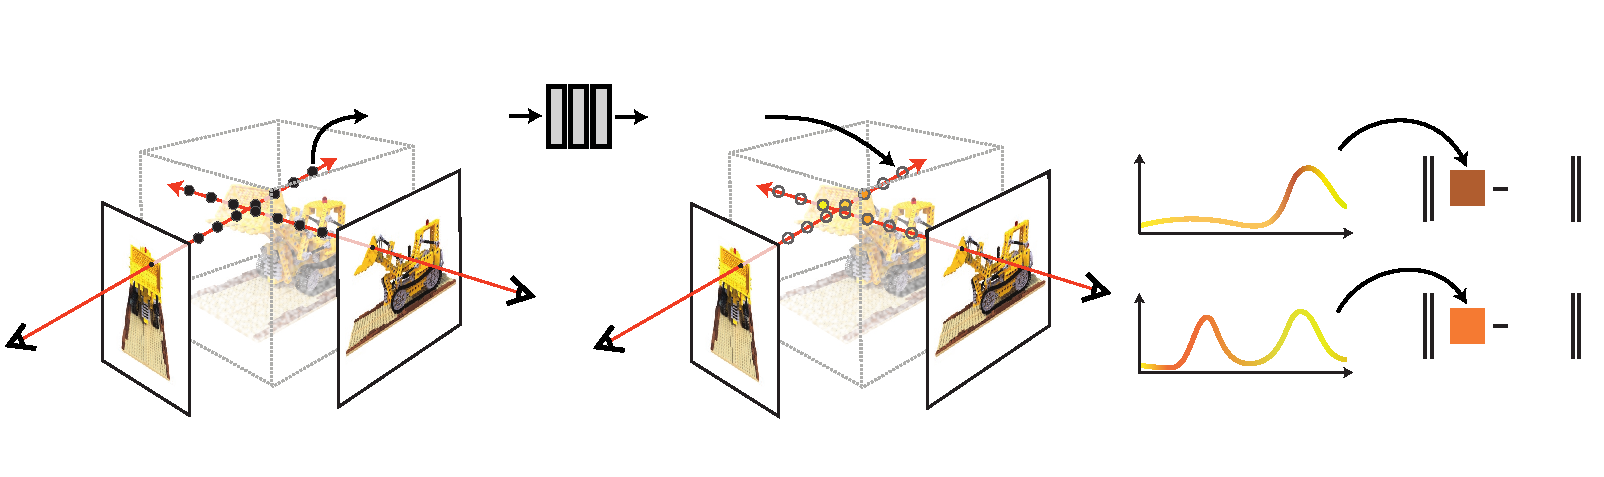
\includegraphics[width=\textwidth]{img/nerf-pipeline.pdf}};
			\begin{scope}[x={(image.south east)},y={(image.north west)}]
				\node[font=\small] at (0.18, 0.9) {Улаз}; 
				\node[font=\small] at (0.54, 0.9) {Излаз};
				\node[font=\small] at (0.771, 0.9) {Рендеровање};
				\node[font=\small] at (0.94, 0.9) {$\mathcal{L}$};
				\node[font=\scriptsize] at (0.7, 0.64) {$\sigma$};
				\node[font=\scriptsize] at (0.7, 0.348) {$\sigma$};
				\node[font=\footnotesize] at (0.273, 0.756) {$(xyz\theta\phi)$};
				\node[font=\scriptsize] at (0.44, 0.756) {$(RGB\sigma)$};
				\node[font=\tiny] at (0.99, 0.67) {2};
				\node[font=\tiny] at (0.99, 0.54) {2};
				\node[font=\tiny] at (0.99, 0.38) {2};
				\node[font=\tiny] at (0.99, 0.25) {2};
				\node[blue,font=\tiny] at (0.775, 0.67) {Зрак 1};
				\node[green,font=\tiny] at (0.775, 0.38) {Зрак 2};
				\node[font=\tiny] at (0.775, 0.18) {Растојање};
				\node[font=\scriptsize] at (0.957, 0.605) {GT};
				\node[font=\scriptsize] at (0.957, 0.32) {GT};
				\node[blue,font=\tiny] at (0.595, 0.695) {Зрак 1};
				\node[green,font=\tiny] at (0.445, 0.61) {Зрак 2};
				\node[font=\small] at (0.362, 0.63) {$f_\Theta$};
			\end{scope}
		\end{tikzpicture}
	\end{center}
	\caption{Илустрација NeRF модела према \cite{nerf}}
	\label{fig-nerf-pipeline}
\end{figure}

\subsection{Параметризација}
Неуронско поље зрачења се параметризује вишеслојним перцептроном, али на благо неуобичајен начин. Јасно је да $\sigma$
не зависи од угла гледања већ искључиво од положаја $\mathbf{x}$. С друге стране, боја пиксела зависи од положаја
као и од пропусности. Зато ReLU MLP од 8 слојева са по 256 неурона на улазу добија само $\mathbf{x}$, док је излаз
предвиђена вредност $\sigma$ и вектор димензије 256. Тај вектор се спаја са параметрима угла гледања и пропушта
кроз један слој са 128 неурона и ReLU aктивационом функцијом. На овај начин се добија боја пиксела која је 
условљена погледом. Поменуте неуронске мреже називамо редом \textit{просторни} и \textit{усмерени} MLP.

Чак и уз овако дефинисан поступак добијања коначног излаза, улаз и даље има малу димензију. Да би се превазишао
тај проблем, улази се прво пресликају у простор веће димензије. Према томе, неуронску мрежу $F_\Theta$ можемо
видети као композицију $F_\theta^\prime \circ \gamma$ где се $\gamma$ не обучава. У овом случају је
$\gamma : \mathbb{R} \rightarrow \mathbb{R}^{2D}$ и то конкретно

\begin{equation}
	\gamma(x) = (\sin(2^0\pi x), \cos(2^0 \pi x), ..., \sin(2^{D-1}\pi x), \cos(2^{D-1}\pi x)).
	\label{eqn-fourier-features}
\end{equation}

Исто пресликавање се користи за све улазе које MLP добија, с тим што се за положај узима $D=10$, a за поглед $D=4$.
Овај начин \textit{подизања} у простор веће димензије није случајан и инспирисан је \cite{transformer}, a могуће
варијације су објашњене у \cite{fourier-coefficients}. Описани поступак се назива \textbf{\textit{Фуријеизација}}.

\subsection{Рендеровање}
У основи је једначина \ref{eqn-volume-rendering-colorimetry}. За потребе апроксимације интеграла биће коришћен
Гаусов метод. Уколико користимо детерминистички приступ, одбирци који учествују у апроксимацији ће увек бити исти.
То је неповољан приступ будући да би у том случају неуронско поље зрачења било увек узорковано за исти скуп
параметара. Уместо тога, увешћемо еквидистантну поделу сегмента $\left[t_n, t_f\right]$, а потом насумице
одабрати по један број из сваког елемента поделе. То формално исказујемо наредним изразом

\begin{equation}
	t_i \sim \mathcal{U}\left[t_n + \frac{i - 1}{N}(t_f - t_n), t_n + \frac{i}{N}(t_f -t_n)\right].
	\label{eqn-uniform-sampling}
\end{equation}

Препишимо једначину \ref{eqn-volume-rendering-colorimetry} у дискретном облику, у складу са
\ref{eqn-uniform-sampling}

\begin{equation}
	\hat{C}(\Pi_{\mathbf{r_{c, d}}}) = \sum_{i=1}^{N} T_i (1- \exp(-\sigma_i\Delta_i)) \mathbf{c}_i,
	\label{eqn-discrete-rendering}
\end{equation}

где је $T_i = \exp\left(-\sum_{j=1}^{i-1}\sigma_j\Delta_j\right)$, парови $(\mathbf{c}_i, \sigma_i)$
одговарајући у складу са избором $t_i$, а $\Delta_i$ ширина елемента поделе.

Једначине \ref{eqn-volume-rendering-colorimetry} и \ref{eqn-discrete-rendering} се видно разликују по
начину на који учествује пропусност. Наиме, уколико би Гаусов метод применили директно, појавио би се
линеаран члан $\sigma_i\Delta_i$. Тај члан је је у апроксимацији замењен експоненцијалним
$1 - \exp(-\sigma_i\Delta_i)$. У наставку ћемо објаснити и зашто \cite{volume-rendering}.

Како узимамо да су на сваком елементу поделе боја и пропусност константни,
једначину \ref{eqn-volume-rendering-colorimetry}  расписујемо у складу са тим. Погледајмо како
произвољни елемент поделе учествује у апроксимацији.
\begin{equation}
	\begin{split}
		\hat{C_i}(\Pi_{\mathbf{r_{c, d}}})
			& = \int_{t_i}^{t_{i + 1}} T(t)\sigma_i c_i dt \\
			& = \int_{t_i}^{t_{i + 1}} \sigma_i c_i \exp\left( -\int_{t_n}^{t} \sigma(\mathbf{r_{c, d}}(s)ds) \right)dt \\
			& = \sigma_i c_i \int_{t_i}^{t_{i + 1}} \exp\left( -\int_{t_n}^{t_i} \sigma(\mathbf{r_{c, d}}(s)ds) \right)
				\exp\left( -\int_{t_i}^{t_{i + 1}} \sigma_i ds \right) dt \\
			& = T_i \sigma_i c_i \int_{t_i}^{t_{i + 1}} \exp(-\sigma_i(t - t_i))dt \\
			& = T_i \sigma_i c_i \frac{\exp(-\sigma_i(t - t_i))}{-\sigma_i} \Biggr|_{t_i}^{t_{i + 1}} \\
			& = T_i (1 - \exp(-\sigma_i \Delta_i)) c_i.
	\end{split}
\end{equation}

\subsection{Обучавање}

Имплементација инспирисана описаним поступком рендеровања је врло неефикасна -- празан простор и прикривени
региони не доприносе рендерованој слици, а непрестано се узоркују. Из тог разлога се користе два неуронска поља,
за \textit{фина} и \textit{груба} предвиђања. Прво се узоркује $N_c$ одбирака на начин објашњен у
\ref{eqn-uniform-sampling} који се потом дају грубом пољу. На основу грубих предвиђања се врши још једно
узорковање, али овог пута боље навођено. Фино узорковање је пристрасније релевантним деловима простора.

Да би то спровели у дело, излаз грубог неуронског поља записујемо као збир боја дуж зрака пондерисаног
непрозирношћу

\begin{equation}
	\hat{C}_c(\Pi_{\mathbf{r_{c, d}}}) = \sum_{i=1}^{N_c}w_i c_i, \quad w_i = T_i (1- \exp(-\sigma_i\Delta_i)).
\end{equation}

Скалирањем тежина $w_i = \nicefrac{w_i}{\sum_{j=1}^{N_c}w_j}$, добија се део-по-део константна густина расподеле дуж зрака.
Из ове расподеле се (инверзно) узоркује $N_f$ oдбирака, а потом фино неуронско поље израчуна у свих
$N_c + N_f$ одбирака на начин описан у једначини \ref{eqn-discrete-rendering}. У свим експериментима се
за $N_c$ узима 64, а за $N_f$ 128. Да би означили о каквом узорковању је реч, увешћемо додатне ознаке
$f$ и $c$.

Функција губитка која се користи за обучавање NeRF-а је
\begin{equation}
	\mathcal{L} = \sum_{\mathbf{r_{c, d}} \in \mathcal{B}}
 	\left(
 	\left\Vert \hat{C}_c\left(\Pi_{\mathbf{r}^{c}_{\mathbf{c}, \mathbf{d}}}\right) -
 		C\left(\Pi_{\mathbf{r}^{c}_{\mathbf{c}, \mathbf{d}}}\right) \right\Vert^2_2 +
	\left\Vert \hat{C}_f\left(\Pi_{\mathbf{r}^{f}_{\mathbf{c}, \mathbf{d}}}\right) -
		C\left(\Pi_{\mathbf{r}^{f}_{\mathbf{c}, \mathbf{d}}}\right) \right\Vert^2_2
	\right).
	\label{eqn-nerf-loss}
\end{equation}

\section{Mip-NeRF}
Као што смо могли да видимо у претходној глави, NeRF jе далеко од идеалног теоријског модела и
показује извесне недостатке. То су постојање два модела који се упоредо обучавају, узорковање
дуж само једног зрака за сваки пиксел, а као што ћемо видети касније у табели \ref{table-duration},
обучавање траје данима. Овом архитектуром покушаћемо да превазиђемо или макар ублажимо наведено.

\begin{figure}[H]
	\begin{center}
		\begin{tikzpicture}
			\node[anchor=south west,inner sep=0] (image) at (0, 0) {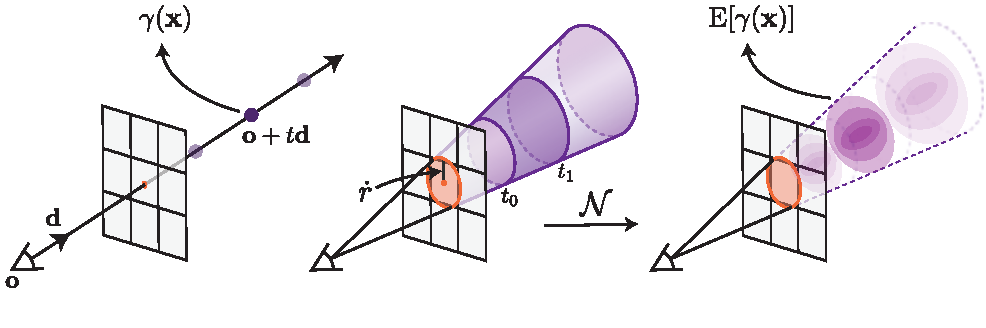
\includegraphics[width=\textwidth]{img/nerf_vs_mipnerf.pdf}};
			\begin{scope}[x={(image.south east)},y={(image.north west)}]
				\node[font=\small] at (0.2, 0) {NeRF};
				\node[font=\small] at (0.6, 0) {mip-NeRF};
				\fill[white] (0.352, 0.36) rectangle (0.377, 0.5);
				\node at (0.365, 0.43) {$R$};
				\fill[white] (0.7, 0.88) rectangle (0.83, 0.99);
				\node at (0.765, 0.945) {$\mathbb{E}(\gamma(\mathbf{x}))$};
			\end{scope}
		\end{tikzpicture}
	\end{center}
	\caption{Поређење NeRF и mip-NeRF модела према \cite{mip-nerf}}
	\label{fig-nerf-vs-mipnerf}
\end{figure}

Кренућемо од кључног недостатка -- постојање само једног зрака по пикселу. Природно проширење
је конусно емитовање зрака. Конус ћемо ограничити двема равнима чиме добијамо зарубљену купу
која је једнозначно одређена центром $\mathbf{o}$, осом симетрије $\mathbf{d}$ и полупречником
круга $R$ који је пресек поменуте купе и равни слике. Скуп тачака које припадају зарубљеној купи
на сегменту параметра $\left[t_0, t_1\right]$ је одређен индикаторском променљивом

\begin{equation}
	\begin{split}
		F(\mathbf{x}, \mathbf{o}, \mathbf{d}, R, t_0, t_1) & =
			I \left(t_0 < \frac{\mathbf{d}^T(\mathbf{x} - \mathbf{o})}{\left\Vert\mathbf{d}\right\Vert^2_2} < t_1 \right) \\
			& \land
			\left(
				\frac{\mathbf{d}^T(\mathbf{x} - \mathbf{o})}
				{\left\Vert\mathbf{d}\right\Vert_2 \left\Vert \mathbf{x} - \mathbf{o}\right\Vert_2}
				> \frac{1}{\sqrt{1 + (R / \left\Vert d\right\Vert_2)^2}}
			\right).
	\end{split}
\end{equation}

\subsection{Интегрална Фуријеизација}
Један од, наизглед, не нарочито битних одлика NeRF-а је допринос Фуријеизације улаза на начин
објашњен у \ref{eqn-fourier-features}. Зато ћемо посебну пажњу посветити управо томе.

Главни циљ је задржати изворну Фуријеизацију. Најједноставнији приступ је одређивање очекиване
изворне Фуријеизације по свим тачкама које припадају купи зрака. Тако добијамо

\begin{equation}
	\gamma^{*}(\mathbf{o}, \mathbf{d}, R, t_0, t_1)
		= \frac{\int\gamma(\mathbf{x})F(\mathbf{x}, \mathbf{o}, \mathbf{d}, R, t_0, t_1)d\mathbf{x}}
				{\int F(\mathbf{x}, \mathbf{o}, \mathbf{d}, R, t_0, t_1)d\mathbf{x}}.
	\label{eqn-ipe-raw}
\end{equation}
Међутим, интеграл који се јавља у овој једначини не умемо да израчунамо. Зато ћемо зарубљену купу
представити нормалном расподелом која нам то омогућава. У ту сврху, потребно је одредити
очекивање и варијансу функције $F(\mathbf{x}, \cdot)$. То за последицу има да је зарубљена купа
апроксимирана елипсоидом, а расподела одређена са пет вредности -- $\mathbf{o}$,
$\mathbf{d}$, $\mu_t$ (очекивано растојање дуж зрака), $\mathbf{\sigma}^2_t$ (варијанса дуж зрака) и
$\mathbf{\sigma}^2_r$ (варијанса дуж нормале зрака).

У наставку ћемо извести засад непознате вредности параметара $\mu_t$, $\sigma_t$ и $\sigma_r$.
Посматрајмо зарубљену купу чија је оса симетрије нормална, односно, паралелна са свим осама.
Употребом сферних координата добијамо параметризацију
\begin{equation}
	(x, y, z) = \phi(r, t, \theta) = (rt\cos\theta, rt\sin\theta, t),
\end{equation}
за $\theta \in [0, 2\pi)$, $t\geq 0$, $|r| \leq R$. Јакобијан је $rt^2drdtd\theta$.

Запремина зарубљене купе је
\begin{equation}
	V = \int_{0}^{2\pi}\int_{t_0}^{t_1}\int_{0}^{R}rt^2drdtd\theta = \pi R \frac{t_1^3 - t_0^3}{3}.
\end{equation}
Расподела у којој се тачке узоркују равномерно из зарубљене купе има густину $rt^2/V$, у шта се можемо
уверити интеграцијом Јакобијана.

Први момент по $t$ је
\begin{equation}
	\begin{split}
		\mathbb{E}(t) & = \frac{1}{V}\int_{0}^{2\pi}\int_{t_0}^{t_1}\int_{0}^{R}t \cdot rt^2drdtd\theta \\
			& = \frac{1}{V}\pi R^2 \frac{t_1^4 - t_0^4}{4} \\
			& = \frac{3(t_1^4 - t_0^4)}{4(t_1^3 - t_0^3)}.
	\end{split}
\end{equation}

Први момент по $x$ (као и по $y$ због симетрије је)
\begin{equation}
	\mathbb{E}(x) = \frac{1}{V}\int_{0}^{2\pi}\int_{t_0}^{t_1}\int_{0}^{R}rt\cos\theta \cdot rt^2drdtd\theta = 0.
\end{equation}

Други момент по $t$ jе
\begin{equation}
	\begin{split}
		\mathbb{E}(t^2) & = \frac{1}{V}\int_{0}^{2\pi}\int_{t_0}^{t_1}\int_{0}^{R}t^2 \cdot rt^2drdtd\theta \\
			& = \frac{1}{V}\pi R^3\frac{t_1^5 - t_0^5}{5} \\
			& = \frac{3(t_1^5 - t_0^5)}{5(t_1^3 - t_0^3)}.
	\end{split}
\end{equation}

Други момент по $x$ (као и по $y$ због симетрије) jе
\begin{equation}
	\begin{split}
		\mathbb{E}(x^2) & = \frac{1}{V}\int_{0}^{2\pi}\int_{t_0}^{t_1}\int_{0}^{R}(rt\cos\theta)^2\cdot rt^2drdtd\theta \\
			& = \frac{1}{V}\frac{R^4}{4}\frac{t_1^5 - t_0^5}{5}\pi \\
			& = \frac{3R^2(t_1^5 - t_0^5)}{20(t_1^3 - t_0^3)}.
	\end{split}
\end{equation}

Када смо израчунали све ове моменте, коначно можемо одредити параметре конусне расподеле који су нам непознати.
Очекивање дуж зрака $\mu_t$ jе први момент по $t$. Варијансу дуж зрака $\sigma_t^2$ добијамо
као $\operatorname{Var}(t) = \mathbb{E}(t^2) - \mathbb{E}(t^2)$. И коначно, $\sigma_r^2 = \mathbb{E}(x^2)$.

У претходним изразима се појављују разлике виших степена, што врло често проузрокује нумеричке потешкоће
када су $t_0$ и $t_1$ блиски. Да то заиста јесте од значаја потврђује чињеница да је апроксимација коју
спроводимо прецизна једино када је зарубљена купа ниска, односно, када је елипсоид нормалне расподеле пљоснат.
Зато се уводе смене $t_\mu = \nicefrac{(t_0 + t_1)}{2}$ и $t_\delta = \nicefrac{(t_1 - t_0)}{2}$.
Коначно, добијамо

\begin{equation}
	\begin{split}
		\mu_t & = t_\mu + \frac{2t_\mu t_\delta^2}{3t_\mu^2 + t_\delta^2} \\
		\sigma_t^2 & = \frac{t_\delta^2}{3} - \frac{4t_\delta^4(12t_\mu^2 - t_\delta^2)}{15(3t_\mu^2 + t_\delta^2)^2} \\
		\sigma_r^2 & = R^2 \left(\frac{t_\mu^2}{4} + \frac{5t_\delta^2}{12} - \frac{4t\delta^4}{15(3t_\mu^2 + t_\delta^2)}\right).
	\end{split}
\end{equation}

На овај начин смо потпуно одредили нормалну расподелу, али у координатном систему равни слике. Међутим,
није тешко доћи до трансформације у светски координатни систем

\begin{equation}
	\begin{split}
		\mu & = \mathbf{o} + \mu_t\mathbf{d} \\
		\Sigma & = \sigma_t^2\left(\mathbf{d}\mathbf{d^T}\right) +
			\sigma_r^2\left(\mathbf{I} - \frac{\mathbf{d}\mathbf{d^T}}{\Vert \mathbf{d}\Vert_2^2}\right).
	\end{split}
\end{equation}

У досадашем разматрању смо припремили терен за дефинисање \textit{интегралне Фуријеизације} која се
прилагођава новоуведеном конусном емитовању зрака. Подсетићемо се идеје још једном -- израчунати очекивану
Фуријеизацију на елипсоиду нормалне расподеле. Дакле, потребно је пресликати улаз у простор више димензије,
а потом у том простору израчунати очекивање. Да би се та два корака ускладила, другачије ћемо записати
\ref{eqn-fourier-features}

\begin{equation}
		P =
		\begin{bmatrix}
			1 & 0 & 0 & 2 & 0 & 0 & ... & 2^{L-1} & 0 & 0 \\
			0 & 1 & 0 & 0 & 2 & 0 & ... & 0 & 2^{L-1} & 0 \\
			0 & 0 & 1 & 0 & 0 & 2 & ... & 0 & 0 & 2^{L-1}
		\end{bmatrix}^T \text{и }
		\gamma(\mathbf{x}) =
		\begin{bmatrix}
			\sin(P\mathbf{x}) \\
			\cos(P\mathbf{x})
		\end{bmatrix}.
\end{equation}

Параметри расподеле се мењају у складу са новим простором, тако да добијамо
$\boldsymbol{\mu}_\gamma = P\boldsymbol{\mu}$. Облик матрице коваријансе следи из њене линеарности.
Наиме, како је $\operatorname{Cov}(A\mathbf{x}, B\mathbf{y}) = A\operatorname{Cov}(\mathbf{x}, \mathbf{y})B^T$,
то је $\Sigma_\gamma = P\Sigma P^T$.

Преостаје да се израчуна очекивање у складу са вишедимензионом расподелом. Потребно је и довољно је показати
понашање очекивања $\gamma(x)$. Прво ћемо показати очекивање у случају једнодимензионе нормалне расподеле, а
потом и у случају који је нама потребан.
\begin{equation}
	\begin{split}
		\mathbb{E}_{x \sim \mathcal{N}(\mu, \sigma^2)}(\sin x) & = \mathbb{E}(\operatorname{Im}\exp(ix)) \\
			& = \operatorname{Im}\mathbb{E}(\exp(ix)) \\
			& = \operatorname{Im}(\phi_{x \sim \mathcal{N}(\mu, \sigma^2)}(1)) \\
			& = \operatorname{Im}\left(\exp\left(i\mu - \frac{\sigma^2}{2}\right)\right) \\
			& = \sin(x)\exp\left(-\frac{\sigma^2}{2}\right)
	\end{split}
\end{equation}
где је функција $\phi_{x \sim \mathcal{N}(\mu, \sigma^2)}(t)$ je карактеристична функција нормалне расподеле.

Аналогно, добијамo $\mathbb{E}_{x \sim \mathcal{N}(\mu, \sigma^2)}(\cos x) = \cos(x)\exp\left(\nicefrac{-\sigma^2}{2}\right)$.
Уколико уопштимо претходно израчунавање, добијамо
\begin{equation}
	\begin{split}
		\gamma(\boldsymbol{\mu}, \Sigma) & = \mathbb{E}_{x \sim \mathcal{N}(\mu, \sigma^2)}(\gamma(x)) \\
			& =
			\begin{bmatrix}
				\sin(\mu_\gamma) \odot \exp(-(1/2)\operatorname{diag}(\Sigma_\gamma)) \\
				\cos(\mu_\gamma) \odot \exp(-(1/2)\operatorname{diag}(\Sigma_\gamma))
			\end{bmatrix},
		\label{eqn-ipe}
	\end{split}
\end{equation}
где је са $\odot$ oзначено Адамарово, члан-по-члан множење.

Начин на који се изводи множење у запису \ref{eqn-ipe} подразумева употребу само дијагоналних елемената матрице
$\Sigma_\gamma$. Израчунавање пуне матрице изискује пуно рачунских операција и места, за чим уопште нема потребе.
С тим у вези, дијагоналне чланове ћемо израчунати директно $\operatorname{diag}(\Sigma_\gamma)
= \left[\operatorname{diag}(\Sigma), 4\operatorname{diag}(\Sigma), ..., 4^{L-1}\operatorname{diag}(\Sigma)\right]^T$ при чему је
\begin{equation}
	\operatorname{diag}(\operatorname{\Sigma}) = \sigma_t^2(\mathbf{d}\odot\mathbf{d}) +
		\sigma_r^2\left(I - \frac{\mathbf{d} \odot \mathbf{d}}{\Vert\mathbf{d}\Vert_2^2}\right)
\end{equation}

На слици \ref{fig-mipnerf-ipe} је приказана разлика у Фуријеизацији у случају NeRF и mip-NeRF модела.

\begin{figure}[H]
	\begin{center}
		\begin{tikzpicture}
			\node[anchor=south west,inner sep=0] (image) at (0, 0) {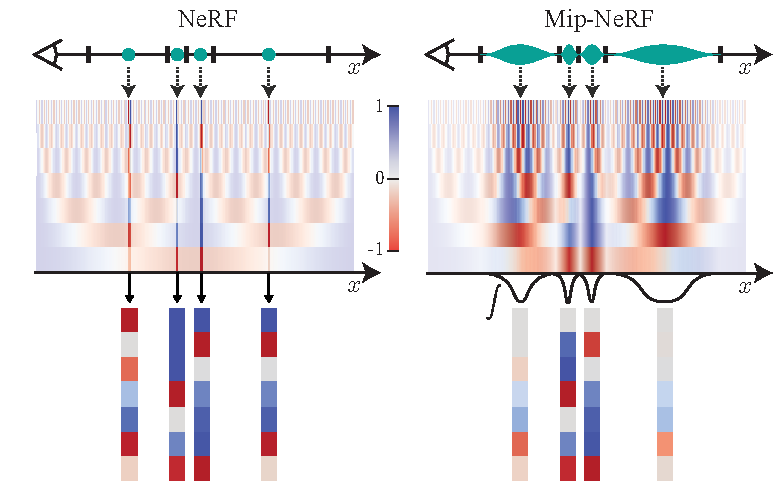
\includegraphics[width=\textwidth]{img/mipnerf_ipe.pdf}};
			\begin{scope}[x={(image.south east)},y={(image.north west)}]
				\fill[white] (0, 0) rectangle (0.04, 1);
				\fill[white] (0, 0.93) rectangle (1, 1);
				\node[rotate=90,font=\scriptsize] at (0.02, 0.88) {oдбирци};
				\node[rotate=90,font=\scriptsize] at (0.02, 0.61) {Фуријеизација};
				\node[rotate=90,font=\scriptsize] at (0.02, 0.2) {Фуријеизовани одбирци};
				\node[font=\small] at (0.25, -0.05) {NeRF};
				\node[font=\small] at (0.75, -0.05) {mip-NeRF};
			\end{scope}
		\end{tikzpicture}
	\end{center}
	\caption{Приказ интегралне Фуријеизације према \cite{mip-nerf}}
	\label{fig-mipnerf-ipe}
\end{figure}

\subsection{Параметризација и обучавање}
Иако mip-NeRF зраке емитује по конусу, обучавање се практично изводи на исти начин као и у случају NeRF-a.
Уместо узорковања $n$ oдбирака дуж зрака, узоркује их се $n+1$ јер ће се узастопно у паровима користити
за границе зарубљене купе. Након примене Фуријеизације, прослеђују се MLP-у и добијају парови $(\sigma, c)$.
MLP je по структури идентичан оном који се користи за параметризацију NeRF-а.

Међутим, mip-NeRF не захтева употребу финог и грубог модела, већ се цео поступак спроводи употребом само једног.
Одговор лежи у употреби конусног емитовања зрака и интегралне Фуријеизације.

Са $\mathbf{k}_{\mathbf{o}, \mathbf{d}, R}$ ћемо означити зарубљену купу са врхом у $\mathbf{o}$, осе
симетрије $\mathbf{d}$ и полупречника пресека купе и равни слике са $R$. Поменути пресек означавамо са
$\Pi_{\mathbf{k}_{\mathbf{o}, \mathbf{d}, R}}$. Ознаке $f$ и $c$ имају исто значење као и у \ref{eqn-nerf-loss}.
Функција губитка која се користи за обучавање mip-NeRF-а је
\begin{equation}
	\mathcal{L} = \sum_{\mathbf{f}_{\mathbf{c}, \mathbf{d}, R} \in \mathcal{B}}
	\left(
	\left\Vert \hat{C}\left(\Pi_{\mathbf{k}^{f}_{\mathbf{c}, \mathbf{d}, R}}\right) -
		C\left(\Pi_{\mathbf{k}^{f}_{\mathbf{c}, \mathbf{d}, R}}\right) \right\Vert^2_2 +
	\lambda
	\left\Vert \hat{C}\left(\Pi_{\mathbf{k}^{c}_{\mathbf{c}, \mathbf{d}, R}}\right) -
		C\left(\Pi_{\mathbf{k}^{c}_{\mathbf{c}, \mathbf{d}, R}}\right) \right\Vert^2_2
	\right).
\end{equation}
Параметар $\lambda$ контролише утицај грубе поделе на функцију губитка јер се само један модел користи за обе врсте поделе.

Врши се укупно по $128$ узорковања за грубу и фину поделу.

\section{Ref-NeRF}
Иако претходне имплементације дају веома добре резултате, за одређене сцене можемо видети њихова ограничења.
Посматрањем резултата на сликама и \ref{fig-materials-results} и \ref{fig-drums-results} можемо уочити проблем
са учењем \textit{сјајности}. Где год постоји изразита спекуларна светлост, NeRF и mip-NeRF нису у стању да је
дочарају верно, већ се стиче утисак дифузне рефлексије -- другим речима, површина делује \textit{обрушено}.

Водећи рачуна о томе како је вектор $\textbf{d}$ усмерен, његову рефлексију око $\textbf{n}$ рачунамо

	\begin{equation}
		\textbf{d}_r = \frac{\textbf{d}}{\left\Vert\mathbf{d}\right\Vert}
		-2\left(\frac{\textbf{d}}{\left\Vert\mathbf{d}\right\Vert} \cdot
			\boldsymbol{\textbf{n}}\right)\textbf{\text{n}}
		\label{eqn-reflection}.
	\end{equation}
о начину добијања поменуте нормале биће више речи касније.

\subsection{Сферна Фуријеизација}
Поново се као кључна разлика јавља другачија врста Фуријеизације, с тим што је овог пута она статистички
заснована. У наставку ћемо објаснити и зашто.

Одаберимо неку тачку на сфери произвољно. Уколико је осветљење сфере у околини те тачке дифузно, тада је
густина одбијених зрака равномернија јер не долази до нагле разлике у осветљењу. С друге стране,
ако је у питању спекуларна рефлексија, тада је расподела одбијених зрака готово Диракова -- приметно
је нагомилавање густине у једној тачки.

Отуда идеја да посматрамо расподелу која добро моделује другачију концентранцију густине у различитим
тачкама на сфери. Зато бирамо \textit{фон Мизес-Фишерову} расподелу. Даћемо формални опис ове
расподеле у случају димензије 3.

	\begin{definition}
		Густина фон Мизес-Фишерове расподеле је дата са
		$$f(\textbf{x}) = \frac{\kappa}{4\pi \sinh\kappa} \exp(\kappa\boldsymbol{\mu}^T\textbf{x)}.$$
		Параметри $\boldsymbol{\mu}$ и $\kappa$ се редом зову \textbf{очекивање} и \textbf{концентрација}.
	\end{definition}

У претходним изведбама смо за потребе пресликавања у простор  више димензије користили Фуријеове коефицијенте,
односно, \textit{хармонике}. Мада се, строго говорећи, хармоници јављају у мало другачијем облику него што је то
случај у Фуријеовом развоју.

Како смо за потребе боље анализе осветљења објекта природно прешли на сферу, а у складу са тим и на одговарајућу
расподелу, хармонике је потребно заменити сферним еквивалентом. Зато уводимо \textit{сферне хармонике}, чији
је приказ дат на слици \ref{fig-refnerf-ide}.

\begin{figure}[H]
	\begin{center}
		\begin{tikzpicture}
			\node[anchor=south west,inner sep=0] (image) at (0, 0) {\includegraphics[width=\textwidth]{img/refnerf_ide.pdf}};
			\begin{scope}[x={(image.south east)},y={(image.north west)}]
				\fill[white] (0, 0) rectangle (0.015, 1);
				\fill[white] (0, 0.93) rectangle (1, 1);
				\fill[white] (0.12, 0.88) rectangle (0.24, 1);
				\node[font=\scriptsize] at (0.18, 0.9) {vMF};
				\node[rotate=90,font=\scriptsize] at (0, 0.73) {спекуларно};
				\node[rotate=90,font=\scriptsize] at (0, 0.22) {дифузно};
				\node[font=\scriptsize] at (0.42, 0.95) {сферни хармоници};
				\node[font=\scriptsize] at (0.82, 0.95) {сферна Фуријеизација};
			\end{scope}
		\end{tikzpicture}
	\end{center}
	\caption{Приказ сферних хармоника и сферне Фуријеизације према \cite{ref-nerf}}
	\label{fig-refnerf-ide}
\end{figure}

	\begin{definition}
		Сферни хармоници су решења Лапласове диференцијалне једначине $\nabla^2f = 0$ у сферним координатама, где је
		$f:\mathbb{R}^3\rightarrow\mathbb{C}$ два пута диференцијабилна функција. Сферни хармоник степена $l$ и реда
		$m$ је комплексна функција на јединичној сфери у ознаци $Y_{l}^{m}$.
	\end{definition}

Следећу теорему наводимо без доказа.

	\begin{theorem}
		Општи облик сферног хармоника $Y_{l}^{m}(\theta, \phi)$ je $Ne^{im\phi}P_{l}^{m}(\cos\theta)$, где је
		$P_{l}^{m}$ одговарајући Лежандров полином, а $N$ коефицијент нормализације. 
	\end{theorem}

	Коефицијент нормализације можемо одредити из ортогоналности. Може се показати да из
	$\int_{S^2}Y_{l}^{m}Y_{l\prime}^{m\prime}dS^2 = 0$, следи
	$$N = \sqrt{\frac{2l + 1}{4\pi}\cdot\frac{(l-m)!}{(l+m)!}}.$$

Претохдно уведене појмове ћемо обједнити \textit{сферном Фуријеизацијом} и то

	\begin{equation}
		\begin{split}
			\gamma(\textbf{d}_r, \kappa) & =
			\{\mathbb{E}_{\boldsymbol{\omega} \sim \operatorname{vMF}(\textbf{d}_r, \kappa)}
			(Y_{l}^{m}(\boldsymbol{\omega})): (l, m) \in \mathcal{M}_L\}, \\
			\text{где је } \mathcal{M}_L & = \{(l, m): l=1, ..., 2^L \land m=0, ..., l\}.
		\end{split}
		\label{eqn-spheric-encoding}
	\end{equation}

Остаје питање израчунавања очекивања
$\mathbb{E}_{\boldsymbol{\omega} \sim \operatorname{vMF}(\textbf{d}_r, \kappa)}(Y_{l}^{m}(\boldsymbol{\omega}))$.
Показује се \cite{ref-nerf} да је поменути израз приближно једнак

	\begin{equation}
		\exp\left(-\frac{l(l+1)}{2\kappa}\right)Y_{l}^{m}(\textbf{d}_r).
	\end{equation}

Иако је изложени теоријски модел расподеле у потпуности оправдан, није јасно како долазимо до параметра концентрације.
Приметимо да је у питању величина обрнуто пропорционална грубости материјала $\rho$. Дифузно осветљење је карактеристично
за делове предмета који нису довољно сјајни, и обратно. Зато користимо идентитет $\kappa = \nicefrac{1}{\rho}$.
За параметар $\rho$ је задужен просторни MLP, о чему ће бити више речи мало касније.

\subsection{Параметризација и обучавање}
Неуронске мреже које чине параметризацију Ref-NeRF-a су у нешто измењеном облику него што смо до сада имали прилике
да видимо. Непосредни излаз просторног MLP-а је сада обогаћен новим величинама. У питању су сви они параметри
на које смо се до сада позивали, али и неке које до сад нисмо имали прилике да поменемо. Према томе,
величине које просторни MLP треба да научи су:

	\begin{itemize}
		\item $\textbf{c}_s$, $\textbf{c}_d$ -- спекуларна и дифузна боја светлости,
		\item \textbf{s} -- нијанса спекуларне светлости,
		\item $\hat{\textbf{n}}$ -- нормала у датој тачки $\textbf{x}$,
		\item \textbf{b} -- латентна репрезентација положаја \textbf{x}. 
	\end{itemize}

Напоменимо још једном да баратамо са посебним величинама које се тичу дифузног и спекуларног осветљења, тј. боја има
своју дифузну и спекуларну компоненту. Остаје да их објединимо у циљу добијања коначне боје. Како дифузно
осветљење зависи само од положаја, користићемо

\begin{equation}
	\textbf{c} = \Gamma(\textbf{c}_d + \textbf{s} \odot \textbf{c}_s),
	\label{eqn-tone}
\end{equation}
где је $\Gamma$ функција преноса у стандардизовани RGB систем \cite{sgrb}.

У oснови овог модела се налази mip-NeRF. За просторни MLP се користи идентична архитектура, али се за потребе усмереног
MLP-а користи 8 слојева са по 256 неурона и ReLU функцијом активације. Приказ архитектуре и редоследа операција је 
дат на слици \ref{fig-refnerf-architecture}.

Обучавање се спроводи на исти начин као и у случају mip-NeRF-a, тако да то нећемо описивати поново.

Међутим, као главна разлика у погледу параметризације између поменутих модела је у већем броју параметара у корист
Ref-Nerf-а. У табели \ref{table-duration} jе приказан њихов однос.

\begin{figure}[h]
	\begin{center}
		\begin{tikzpicture}[style={align=center}]
			\definecolor{lightblue}{RGB}{235,243,255}
			\definecolor{lightyellow}{RGB}{255,250,223}
			\node[anchor=south west,inner sep=0] (image) at (0, 0) {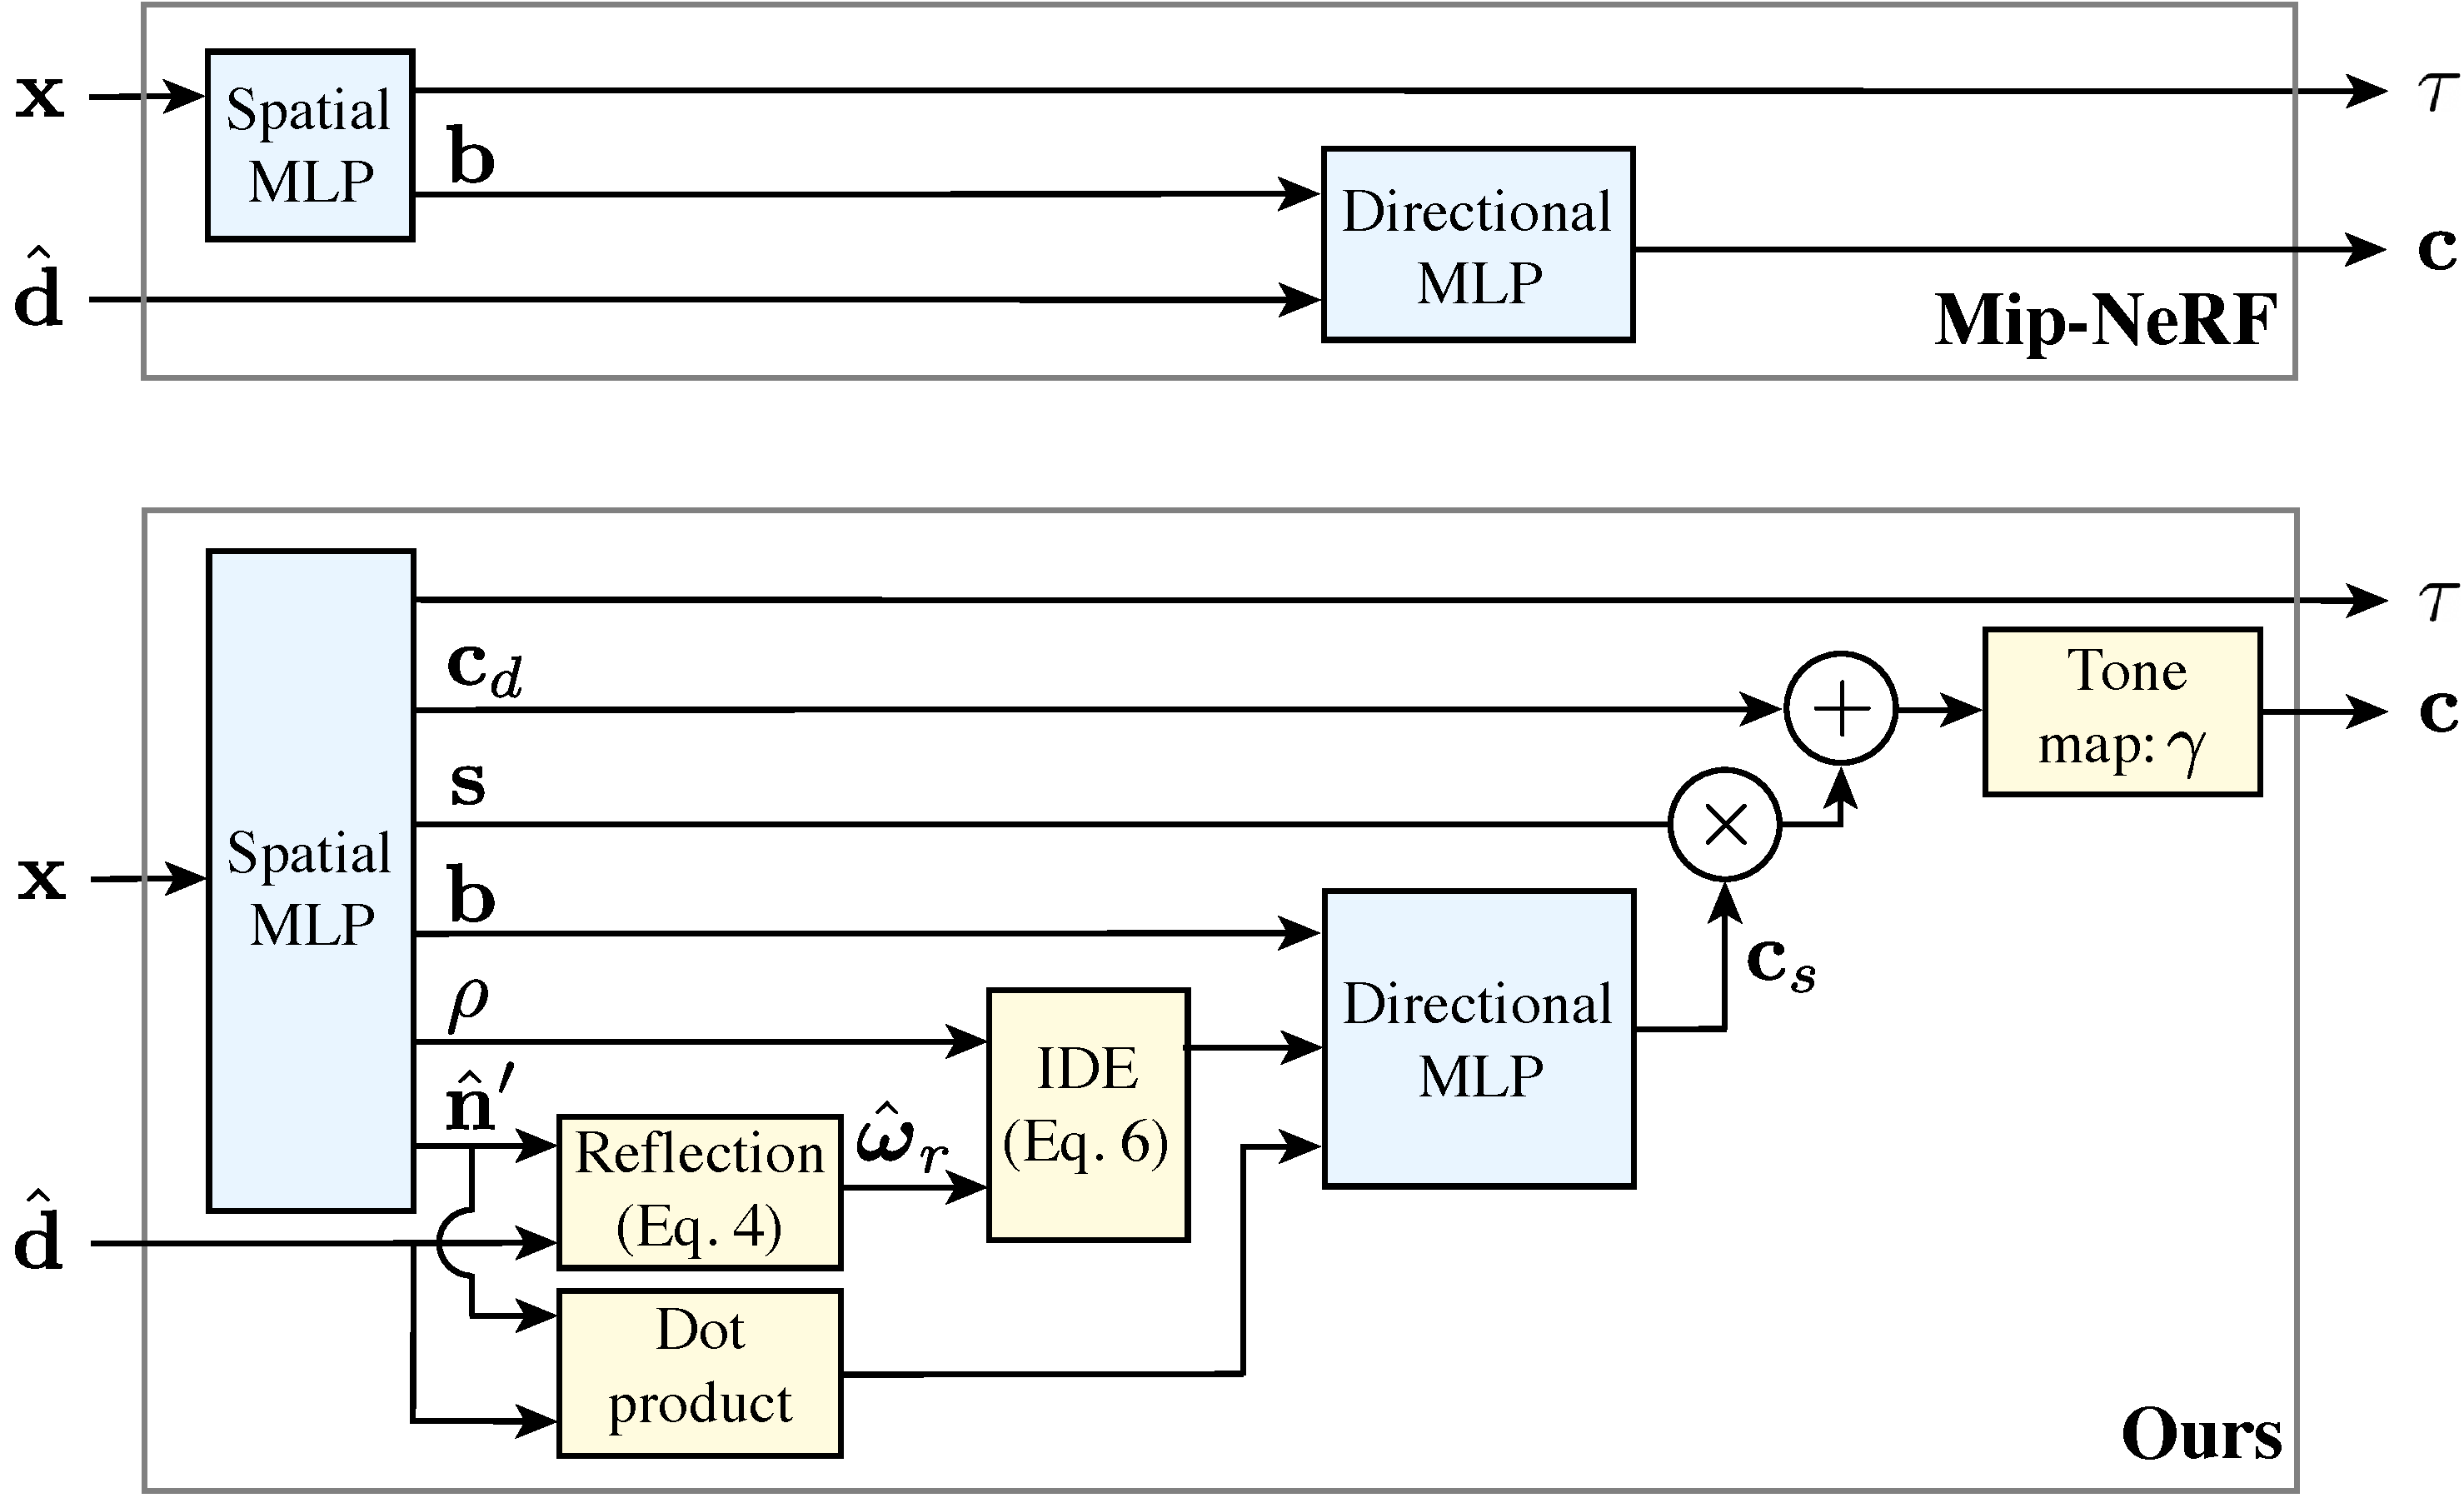
\includegraphics[width=\textwidth]{img/refnerf-architecture.pdf}};
			\begin{scope}[x={(image.south east)},y={(image.north west)}]
				\fill[lightblue] (0.09, 0.85) rectangle (0.16, 0.95);
				\fill[lightblue] (0.09, 0.6) rectangle (0.16, 0.2);
				\fill[lightblue] (0.54, 0.25) rectangle (0.66, 0.4);
				\fill[lightyellow] (0.23, 0.16) rectangle (0.335, 0.25);
				\fill[lightyellow] (0.23, 0.04) rectangle (0.335, 0.13);
				\fill[lightyellow] (0.405, 0.18) rectangle (0.475, 0.33);
				\fill[lightyellow] (0.82, 0.48) rectangle (0.9, 0.57);
				\fill[white] (0.78, 0.75) rectangle (0.925, 0.83);
				\node[font=\small] at (0.127, 0.9) {Прост. \\ MLP};
				\node[font=\small] at (0.127, 0.41) {Прост. \\ MLP};
				\node[font=\small,fill=lightblue] at (0.6, 0.835) {Усмерени \\ MLP};
				\node[font=\small,fill=lightblue] at (0.601, 0.31) {Усмерени \\ MLP};
				\node[font=\large] at (0.855, 0.775) {mip-NeRF};
				\node[font=\large,fill=white] at (0.855, 0.04) {Ref-NeRF};
				\node[font=\large] at (0.86, 0.52) {\ref{eqn-tone}};
				\node[font=\large] at (0.443, 0.25) {\ref{eqn-spheric-encoding}};
				\node[font=\scriptsize] at (0.285, 0.08) {Скаларни \\ производ};
				\node[font=\large] at (0.285, 0.205) {\ref{eqn-reflection}};
				\fill[white] (0.2, 0.25) rectangle (0.21, 0.3);
				\fill[white] (0.345, 0.225) rectangle (0.385, 0.281);
				\fill[white] (0.01, 0.195) rectangle (0.021, 0.21);
				\fill[white] (0.01, 0.825) rectangle (0.021, 0.84);
				
				\node[font=\large] at (0.37, 0.24) {$\textbf{d}_r$};
%				\fill[white] (0.35, 0.255) rectangle (0.37, 0.28);
			\end{scope}
		\end{tikzpicture}
	\end{center}
	\caption{Поређење mip-NeRF и Ref-NeRF aрхитектура}
	\label{fig-refnerf-architecture}
\end{figure}

\subsection{Израчунавање вектора нормале}
Вектор нормале у некој тачки се тривијално рачуна из усмереног MLP-а. Може се користити идентитет
	\begin{equation}
		\hat{\textbf{n}}(\textbf{x}) = -\frac{\nabla\tau(\textbf{x})}{\left\Vert\nabla\tau(x)\right\Vert}.
	\end{equation}
Међутим овај метод је изузетно непрецизан јер се од самог почетка ослања на недовољно обучен усмерени модел.

%\section{Instant-NGP}
%\begin{figure}[H]
%	\begin{center}
%		\begin{tikzpicture}
%			\node[anchor=south west,inner sep=0] (image) at (0, 0) {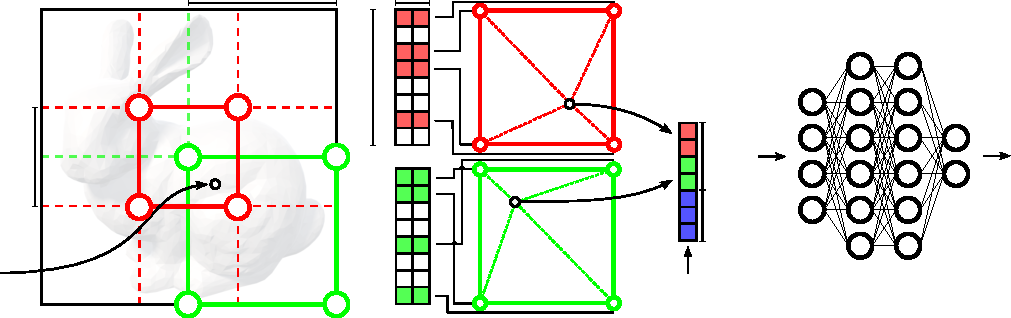
\includegraphics[width=\textwidth]{img/instantngp-pipeline.pdf}};
%			\begin{scope}[x={(image.south east)},y={(image.north west)}]
%				\node[font=\scriptsize] at (0.19, 1.15) {Хеширање};
%				\node[font=\scriptsize] at (0.54, 1.15) {Интерполација};
%				\node[font=\scriptsize] at (0.69, 1.15) {Конкатенација};
%				\node[font=\scriptsize] at (0.01, 0.505) {$1/N_1$};
%				\node[font=\tiny] at (0.1862, 0.506) {0};
%				\node[font=\tiny] at (0.1862, 0.045) {1};
%				\node[font=\tiny] at (0.333, 0.506) {4};
%				\node[font=\tiny] at (0.333, 0.045) {7};
%				\node[font=\tiny] at (0.236, 0.3475) {6};
%				\node[font=\tiny] at (0.138, 0.3475) {3};
%				\node[font=\tiny] at (0.138, 0.663) {2};
%				\node[font=\tiny] at (0.236, 0.663) {0};
%				\node[font=\scriptsize] at (0.68, 0.10) {$\xi$};
%				\node[font=\tiny] at (0.715, 0.51) {$L \cdot F$};
%				\node[font=\tiny] at (0.703, 0.33) {$E$};
%				\node[font=\scriptsize] at (0.877, 0.88) {$f_\Theta$};
%				\node[font=\scriptsize] at (-0.008, 0.142) {$\mathrm{x}$};
%				\node[font=\scriptsize] at (0.41, 1.02) {$F$};
%				\node[font=\scriptsize] at (0.357, 0.76) {$T$};
%				\node[font=\scriptsize] at (0.26, 1.03) {$1/N_0$};
%				\node[red,font=\tiny] at (0.205, 0.69) {$l=1$};
%				\node[green,font=\tiny] at (0.302, 0.534) {$l=0$};
%				\node[font=\tiny] at (0.385, 0.942) {0};
%				\node[font=\tiny] at (0.385, 0.89) {1};
%				\node[font=\tiny] at (0.385, 0.836) {2};
%				\node[font=\tiny] at (0.385, 0.783) {3};
%				\node[font=\tiny] at (0.385, 0.73) {4};
%				\node[font=\tiny] at (0.385, 0.677) {5};
%				\node[font=\tiny] at (0.385, 0.625) {6};
%				\node[font=\tiny] at (0.385, 0.57) {7};
%			\end{scope}
%		\end{tikzpicture}
%	\end{center}
%	\caption{Илустрација Instant-NGP модела према \cite{instant-ngp}}
%	\label{fig-instantngp-pipeline}
%\end{figure}

\chapter{Скупови података}
Скупови података у области неуронских поља зрачења се угрубо могу поделити на две групе -- да ли је позната
калибрација камере или не. У овом раду смо се опредили за прву групу. Разлози су  пре свега техничке природе.
Проблем калибрације камере је један од централних проблема рачунарског вида и као такав је добро испитан.
Може се рећи да је овај проблем \textit{лоше условљен}. Готово незнатне разлике могу довести до значајних грешака
у пројекцијама, а врло прецизна калибрација изискује и скупу опрему. Олакшавајућа околност је да су познати поступци
одређивања унутрашњих и спољашњих параметара камере, али јасно је да они не могу бити ни близу прецизни као што је,
на пример, роботска калибрација. С тим у вези, мишљења смо да је оправдано користити синтетички генерисане скупове
података у којима ће камера бити постављена на унапред одређено место, а сви њени параметри ће бити познати по дефиницији.

За потребе овог рада, коришћени су \textsc{Lego}, \textsc{Materials}, \textsc{Drums}, \textsc{Chair} и \textsc{Ship}.
У питању су познати, референтни скупови података. Модели ће бити упоређени на сваком од њих у истом окружењу.
Конкретно, у питању су редом багер од Лего коцки, 16 лоптица различитих материјала, бубњеви, столица и брод.
На слици \ref{fig-datasets} је приказан по један поглед за сваки од скупова.

Сваки скуп података је подељен на три подскупа -- за обучавање, проверу и тестирање. У подскуповима за обучавање и проверу
се налази тачно 100 rазличитих погледа, док се за тестирање користи 200. Рендери су синтетички, резолуције 800$\times$800
пиксела без радијалне и тангенцијалне дисторзије.

\begin{figure}[H]
	\centering
	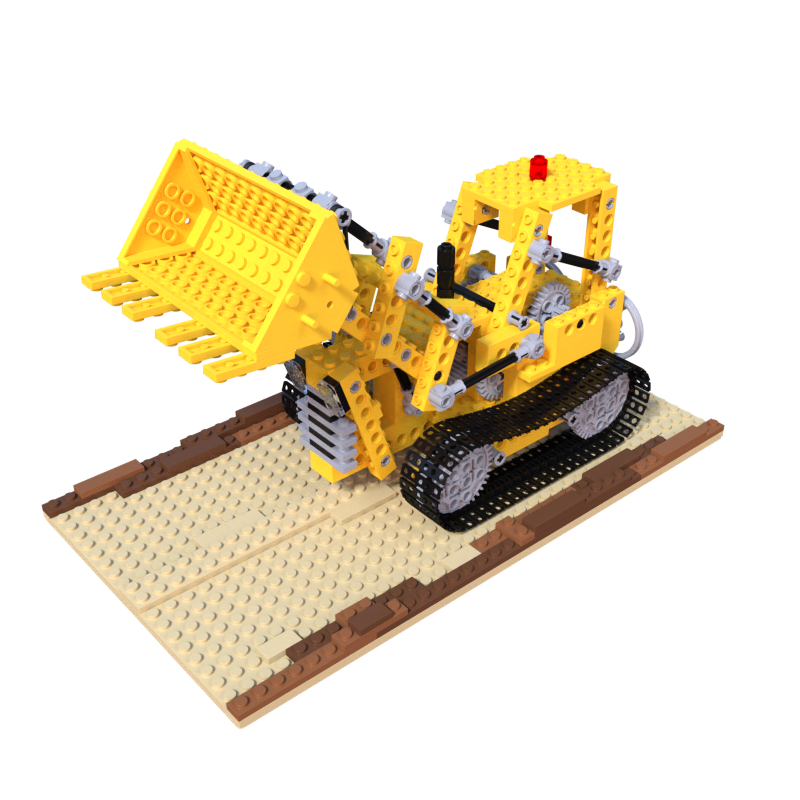
\includegraphics[width=.3\textwidth]{img/lego_gt.png}\quad
	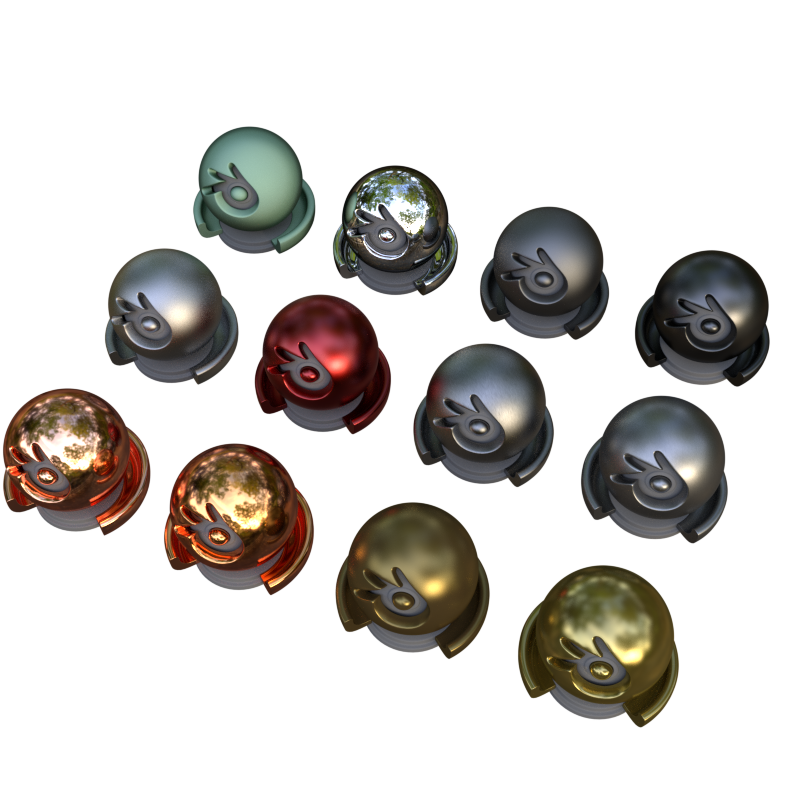
\includegraphics[width=.3\textwidth]{img/materials_gt.png}\quad
	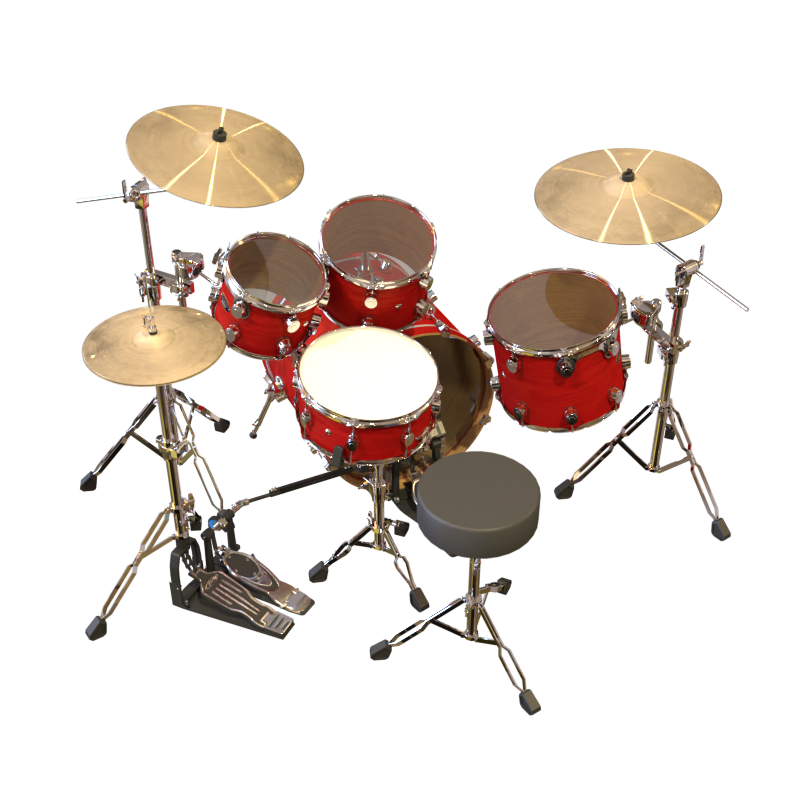
\includegraphics[width=.3\textwidth]{img/drums_gt.png}
	\medskip
	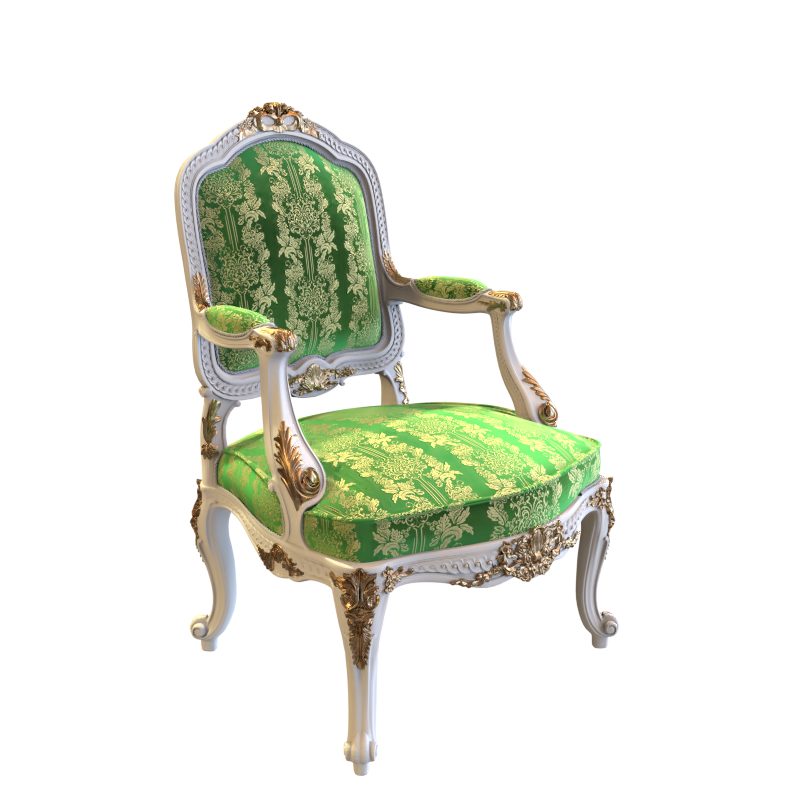
\includegraphics[width=.3\textwidth]{img/chair.png}\quad
	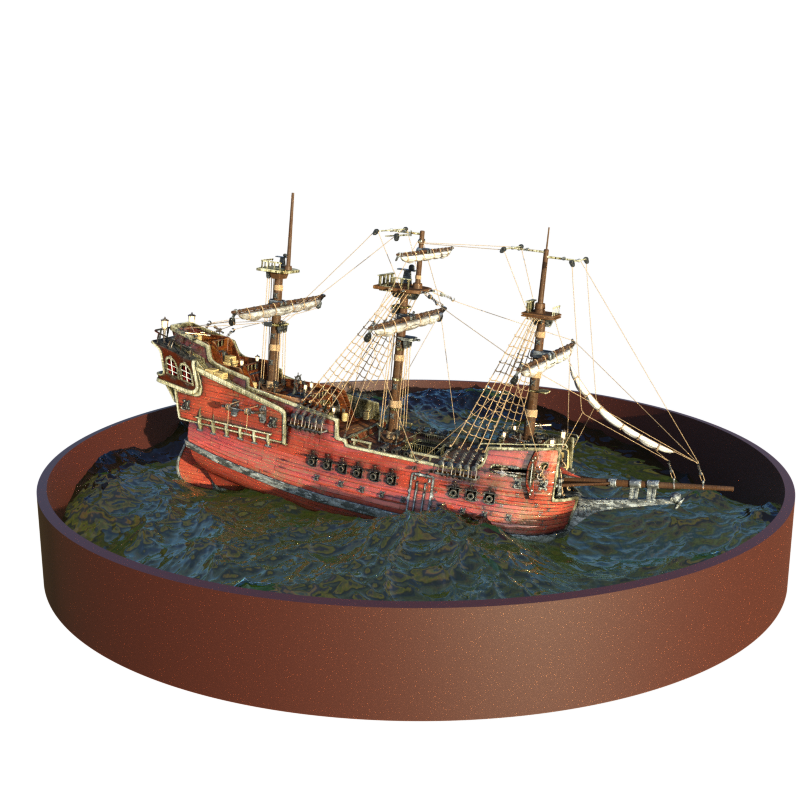
\includegraphics[width=.3\textwidth]{img/ship_gt.png}
	\caption{По један поглед из сваког скупа података}
	\label{fig-datasets}
\end{figure}

\chapter{Експерименти}
Модели ће бити упоређени по свакој од метрика које ћемо навести и објаснити у наставку. Такође, како је дужина
трајања обучавања од великог значаја, посебну пажњу ћемо посветити и том аспекту.

Обучавање је вршено употребом сервиса AzureML са избором параметара у складу са изворним радовима, са само једним
изузетком -- параметар \texttt{batch\_size} је мањи услед просторних ограничења. Графички процесор који је коришћен
носи ознаку NVIDIA Tesla K80 са 24GB сопствене меморије. Имплементација је изведена у програмском језику Python
користећи PyTorch \cite{pytorch}.

Поштовани су изворни избори параметара, са само једним изузетком -- параметар \texttt{batch\_size} је мањи
услед просторних ограничења.

\section{Метрике}
\noindent \textbf{PSNR} (eнг. \textit{Peak Signal-to-Noise Ratio}). Нека је дата монохроматска слика $I$ и њена
апроксимација $K$. Средњеквадратно одступање ове две слике је

\begin{equation}
	\text{MSE} = \frac{1}{mn} \sum_{i=0}^{m-1}\sum_{j=0}^{n-1}(I_{i, j} - K_{i, j})^2.
\end{equation}

Однос сигнала и шума је

\begin{equation}
	\text{PSNR} = 10\log_{10}\left(\frac{I_{\max}^2}{\text{MSE}}\right) \left[\text{dB}\right],
\end{equation}
где је $I_{\max}$ највећа могућа вредност коју пиксел на слици може имати. Како се канал слике обично
представља једним бајтом, ова вредност у већини случајева износи 255.

Више вредности ове метрике указују на бољу апроксимацију. \\

\noindent \textbf{LPIPS} (енг. \textit{Learned Perceptual Image Patch Similarity}) \cite{lpips}. Идеја је имати метрику
која опонаша људску процену сличности две слике. У ту сврху се користи модел $\mathcal{F}$ обучен на сликовном
скупу података. Не постоје никаква ограничења у погледу архитектуре, па чак ни скупа података, али се показује да
VGG \cite{vgg} и AlexNet \cite{alexnet} у комбинацији са ImageNet-ом врло добро раде у пракси.

Означимо са $I$ троканалну слику, а са $K$ њену апроксимацију. Иако слојеви  модела $\mathcal{F}$
не морају имати ни улаз ни излаз димензије 2, у овом тренутку ће бити лакше да претпоставимо да то јесте случај. Пре
свега из рачунских разлога. Уколико $\mathcal{F}$ захтева тензоре неке друге димензије, увек се томе можемо прилагодити
једноставним преобличавањем.

Нека је $\boldsymbol{\alpha}_{i, j, k}^{I}$ резултат примене активационе функције у слоју $k$ у врсти
$i$ и колони $j$ за улазну слику $I$. Ове вредности су нормализоване канал по канал. Аналогно имамо и
$\boldsymbol{\alpha}_{i, j, k}^{K}$.

\begin{equation}
	\text{LPIPS} = \sum_{k=1}^{L}\frac{1}{N_i N_j}\sum_{i=0}^{N_i - 1}\sum_{j=0}^{N_j - 1}
	\left\Vert w_k \cdot (\boldsymbol{\alpha}_{i, j, k}^{I} - \boldsymbol{\alpha}_{i, j, k}^{K}) \right\Vert^2.
\end{equation}

Ниже вредности ове метрике указују на бољу апроксимацију. \\

\noindent \textbf{SSIM} (eнг. \textit{Structual Similarity Index Measure}) \cite{ssim}.  Нека је дата монохроматска
слика $I$ и њена апроксимација $K$.
\begin{equation}
	\text{SSIM} = \frac{(2\mu_{I}\mu_{K} + c_1)(2\sigma_{I, K} + c_2)}{(\mu_{I}^2 + \mu_{K}^2 + c_1)(\sigma_{I}^2 + \sigma_{K}^2 + c_2)},
\end{equation}
где су $\mu_{I}$ и $\mu_{K}$ узорачке средине, $\sigma_{I}^2$ и $\sigma_{K}^2$ узорачке дисперзије, а $\sigma_{I, K}$
узорачка коваријанса између $I$ и $K$. Вредности $c_i$ су дефинисане као $(k_i I_{\max})^2$, где је су $k_i$ константе
и то обично редом $0.01$ и $0.03$.

У пракси се показује да овако дефинисана метрика неће дати увек задовољавајуће резултате. Зато се она ретко примењује
на целој слици, већ се слика дели на мање делове, а резултати метрике потом упросече.

Више вредност ове метрике указују на бољу апроксимацију.

\section{Резултати}

	\begin{table}[H]
		\centering
		\begin{tabular}{cccc} \toprule
			{mодел}			& {PSNR $\uparrow$}	& {LPIPS $\downarrow$}	& {SSIM $\uparrow$} \\ \midrule
			{NeRF}			& 34.38				& 0.032					& 0.973 \\ 
			{mip-NeRF}		& \textbf{35.80}	& 0.026					& 0.978 \\
			{Ref-NeRF}		& 35.79				& \textbf{0.024}		& \textbf{0.979} \\ \bottomrule
		\end{tabular}
		\caption{Резулати за \textsc{Lego} скуп података}
		\label{table-lego}
	\end{table}

	\begin{table}[H]
		\centering
		\begin{tabular}{cccc} \toprule
			{mодел}			& {PSNR $\uparrow$} & {LPIPS $\downarrow$}	& {SSIM $\uparrow$} \\ \midrule
			{NeRF} 			& 30.45 			& 0.055					& 0.956 \\ 
			{mip-NeRF}		& 30.58 			& 0.052					& 0.958 \\
			{Ref-NeRF}		& \textbf{35.71}	& \textbf{0.028}		& \textbf{0.985} \\ \bottomrule
		\end{tabular}
		\caption{Резулати за \textsc{Materials} скуп података}
		\label{table-materials}
	\end{table}

	\begin{table}[H]
		\centering
		\begin{tabular}{cccc} \toprule
			{mодел}			& {PSNR $\uparrow$} & {LPIPS $\downarrow$}	& {SSIM $\uparrow$} \\ \midrule
			{NeRF}			& 25.28				& 0.080 				& 0.929 \\ 
			{mip-NeRF}		& \textbf{25.52}	& 0.079					& 0.932 \\
			{Ref-NeRF}		& \textbf{25.52}	& \textbf{0.073}		& \textbf{0.934} \\ \bottomrule
		\end{tabular}
		\caption{Резулати за \textsc{Drums} скуп података}
		\label{table-drums}
	\end{table}

	\begin{table}[H]
		\centering
		\begin{tabular}{cccc} \toprule
			{mодел} 		& {PSNR $\uparrow$} & {LPIPS $\downarrow$}	& {SSIM $\uparrow$} \\ \midrule
			{NeRF} 			& 34.93				& 0.029					& 0.979 \\ 
			{mip-NeRF} 		& 35.20				& 0.028					& 0.981 \\
			{Ref-NeRF}		& \textbf{35.84}	& \textbf{0.022}		& \textbf{0.984} \\ \bottomrule
		\end{tabular}
		\caption{Резулати за \textsc{Chair} скуп података}
		\label{table-chair}
	\end{table}

	\begin{table}[H]
		\centering
		\begin{tabular}{cccc} \toprule
			{mодел}			& {PSNR $\uparrow$} & {LPIPS $\downarrow$}	& {SSIM $\uparrow$} \\ \midrule
			{NeRF}			& 29.94				& 0.161					& 0.878 \\ 
			{mip-NeRF}		& \textbf{30.53} 	& \textbf{0.154}		& \textbf{0.884} \\
			{Ref-NeRF}		& 29.50				& 0.164					& 0.871 \\ \bottomrule
		\end{tabular}
		\caption{Резулати за \textsc{Ship} скуп података}
		\label{table-ship}
	\end{table}

\section{Време обучавања}

Дужина трајања обучавања не зависи од скупа података, a сви модели су обучавани тачно одређен број итерација.

	\begin{table}[H]
		\centering
		\begin{tabular}{cccc} \toprule
			{mодел} 	& {време обучавања (у сатима)} 	& {број итерација} & {број параметара} \\ \midrule
			{NeRF} 		& 120 							& 1000000 & 1200000\\ 
			{mip-NeRF} 	& 127 							& 1000000 & 612000\\
			{Ref-NeRF} 	& 135 							& 1000000 & 1100000\\ \bottomrule
		\end{tabular}
		\caption{Време обучавања за сваки модел}
		\label{table-duration}
	\end{table}


\section{Квалитет резултата}

	\begin{figure}[H]
		\centering
		\begin{subfigure}{0.475\textwidth}
			\centering
			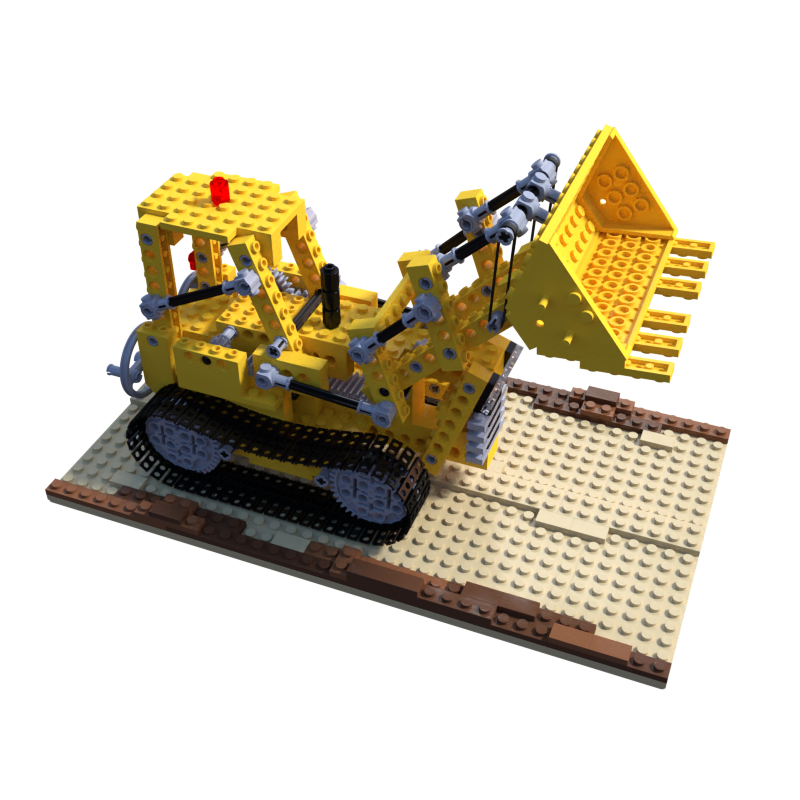
\includegraphics[scale=0.25]{img/gt/gt_lego_31.png}
			\caption{GT}
		\end{subfigure}
		\begin{subfigure}{0.475\textwidth}
			\centering
			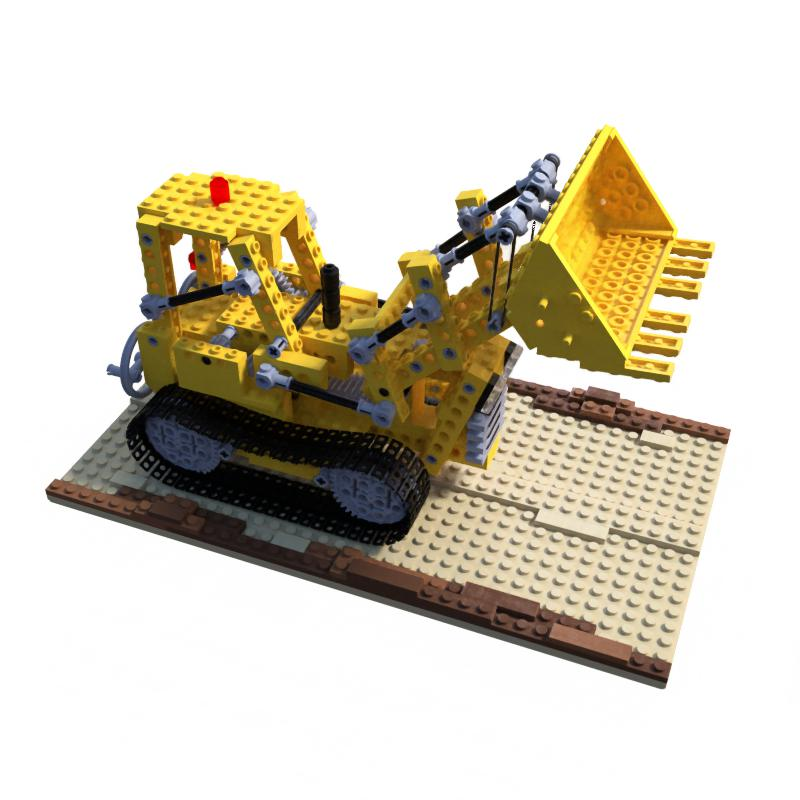
\includegraphics[scale=0.25]{img/nerf/nerf_lego_31.jpg}
			\caption{NeRF}
		\end{subfigure}
		\begin{subfigure}{0.475\textwidth}
			\centering
			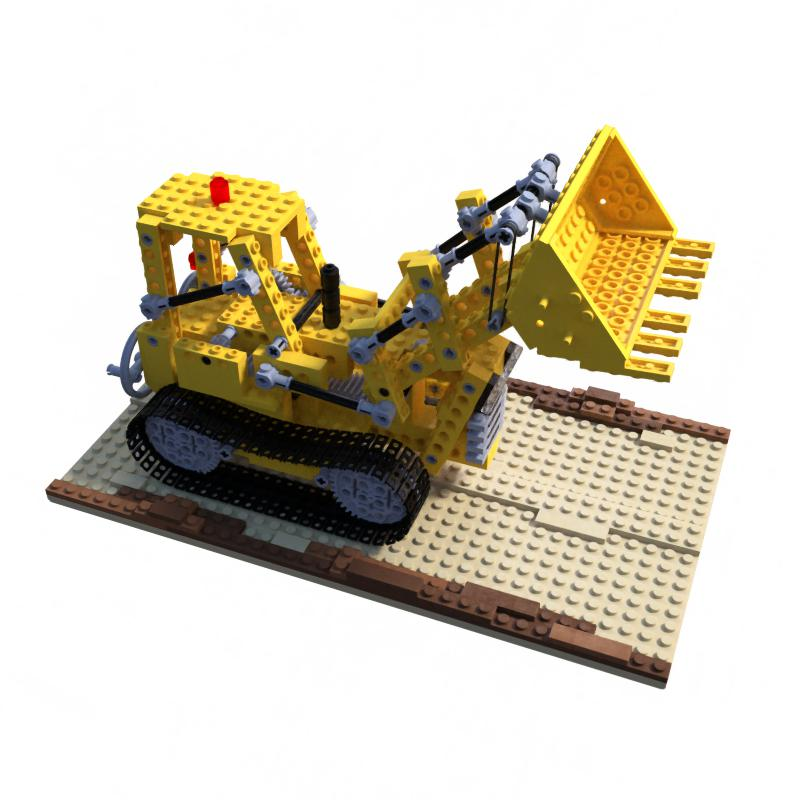
\includegraphics[scale=0.25]{img/mipnerf/mipnerf_lego_31.jpg}
			\caption{mip-NeRF}
		\end{subfigure}
		\begin{subfigure}{0.475\textwidth}
			\centering
			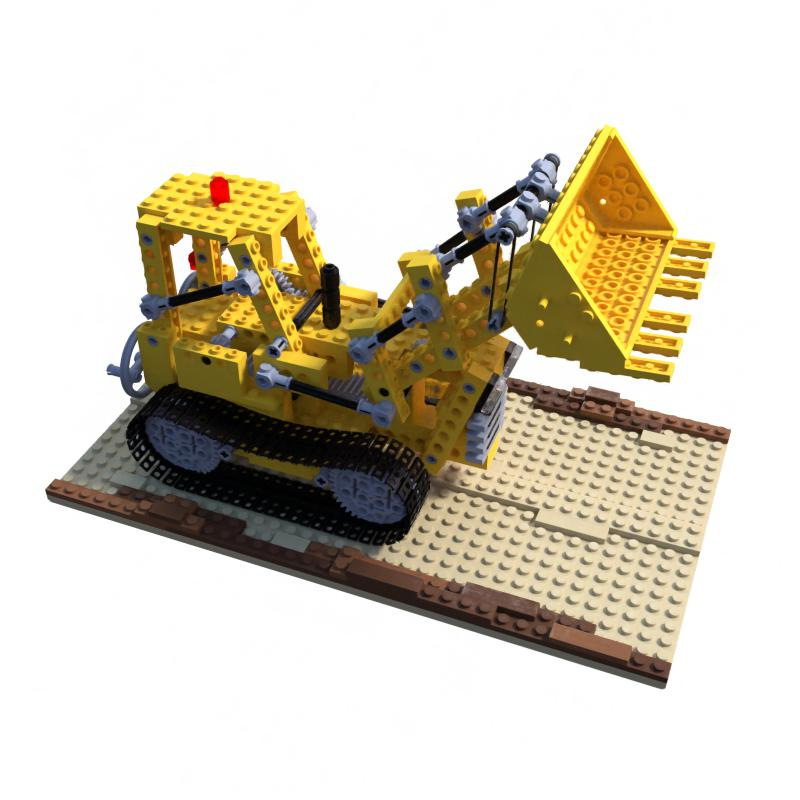
\includegraphics[scale=0.25]{img/refnerf/refnerf_lego_31.jpg}
			\caption{Ref-NeRF}
		\end{subfigure}
		\caption{Приказ резултата \textsc{Lego} скупа података}
		\vspace{5in}
		\label{fig-lego-results}
	\end{figure}

	\begin{figure}[H]
		\centering
		\begin{subfigure}{0.475\textwidth}
			\centering
			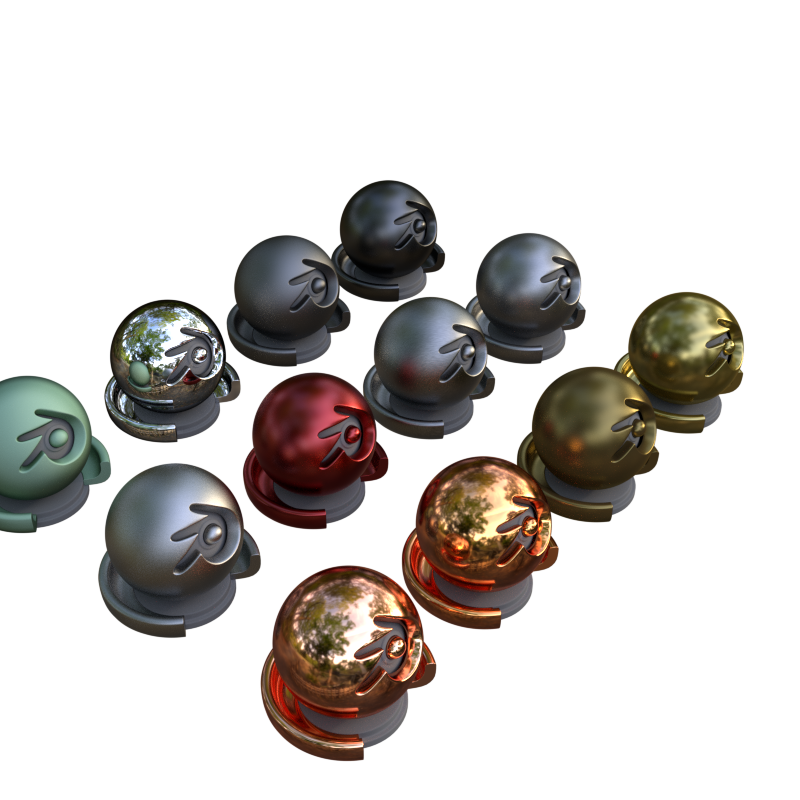
\includegraphics[scale=0.25]{img/gt/gt_materials_36.png}
			\caption{GT}
		\end{subfigure}
		\begin{subfigure}{0.475\textwidth}
			\centering
			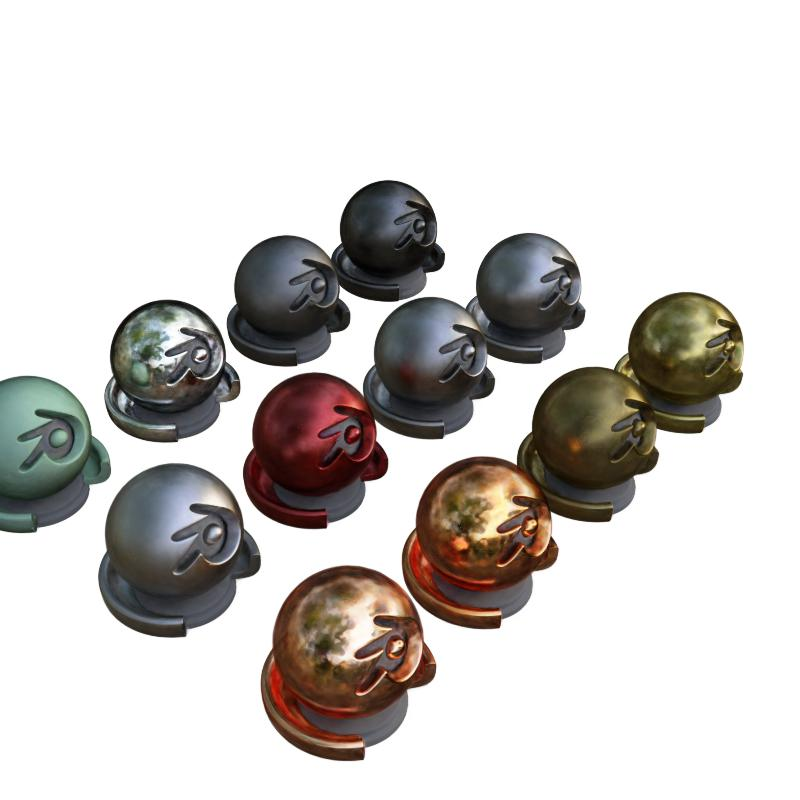
\includegraphics[scale=0.25]{img/nerf/nerf_materials_36.jpg}
			\caption{NeRF}
		\end{subfigure}
		\begin{subfigure}{0.475\textwidth}
			\centering
			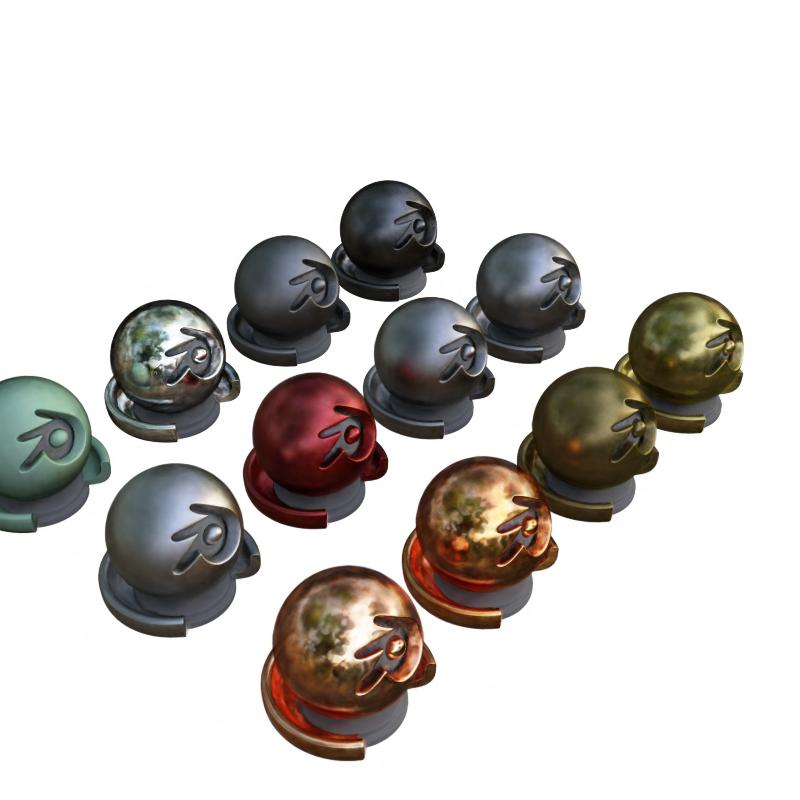
\includegraphics[scale=0.25]{img/mipnerf/mipnerf_materials_36.jpg}
			\caption{mip-NeRF}
		\end{subfigure}
		\begin{subfigure}{0.475\textwidth}
			\centering
			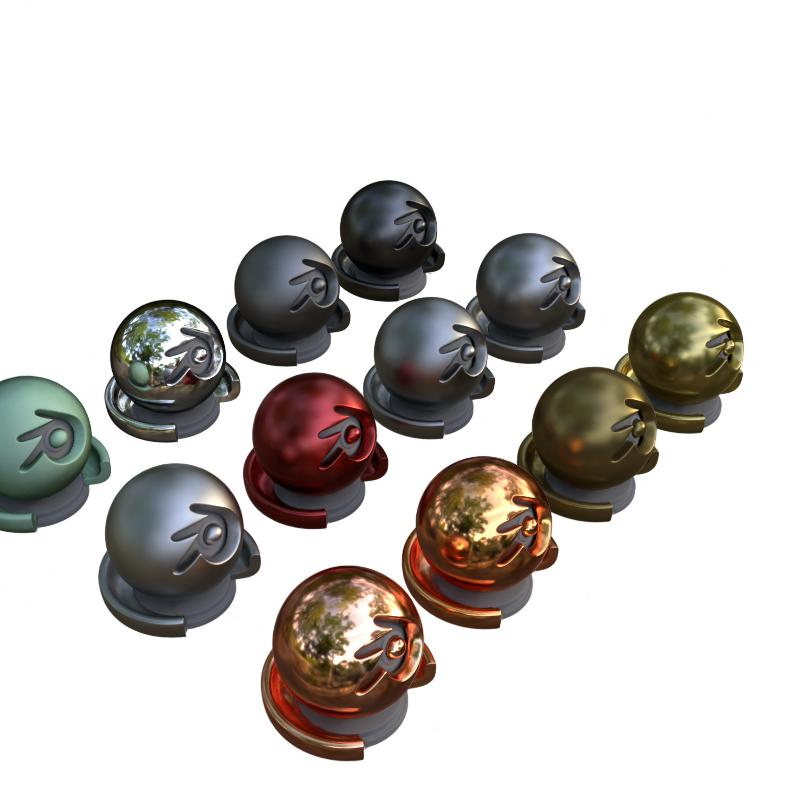
\includegraphics[scale=0.25]{img/refnerf/refnerf_materials_36.jpg}
			\caption{Ref-NeRF}
		\end{subfigure}
		\caption{Приказ резултата \textsc{Materials} скупа података}
		\label{fig-materials-results}
	\end{figure}

	\begin{figure}[H]
		\centering
		\begin{subfigure}{0.475\textwidth}
			\centering
			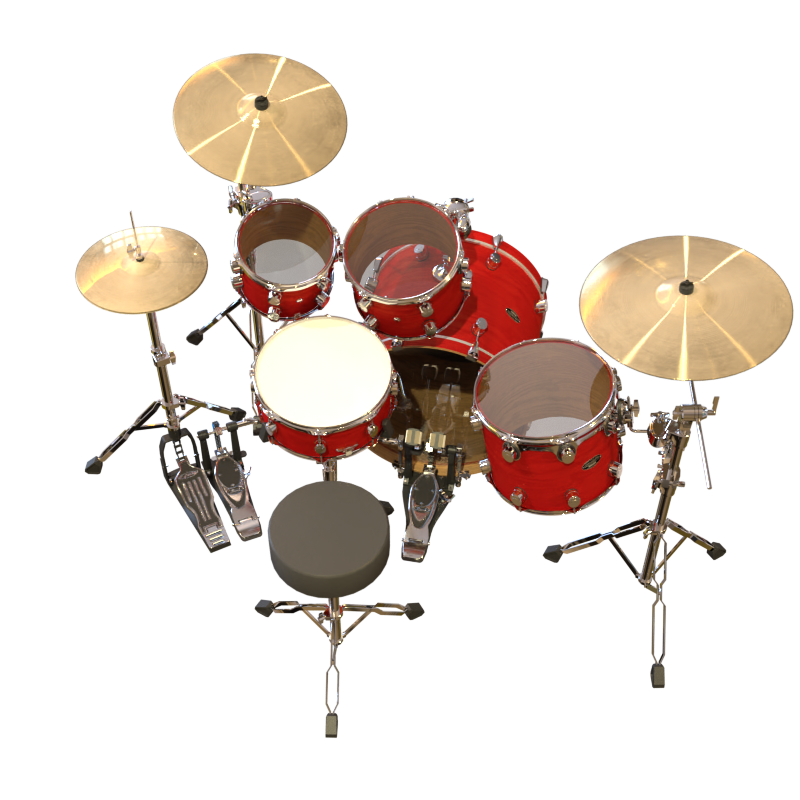
\includegraphics[scale=0.25]{img/gt/gt_drums_3.png}
			\caption{GT}
		\end{subfigure}
		\begin{subfigure}{0.475\textwidth}
			\centering
			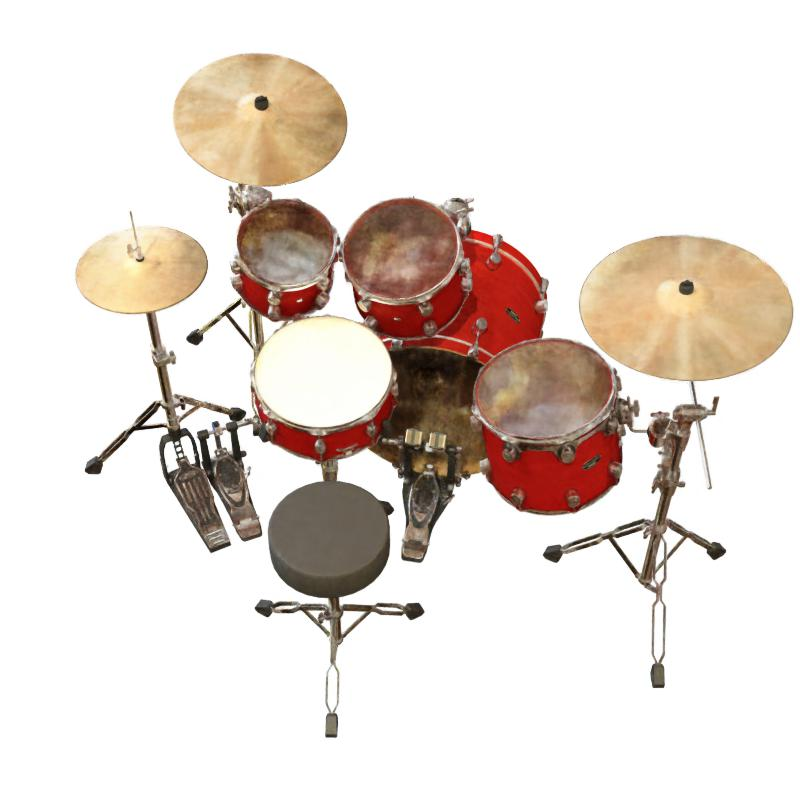
\includegraphics[scale=0.25]{img/nerf/nerf_drums_3.jpg}
			\caption{NeRF}
		\end{subfigure}
		\begin{subfigure}{0.475\textwidth}
			\centering
			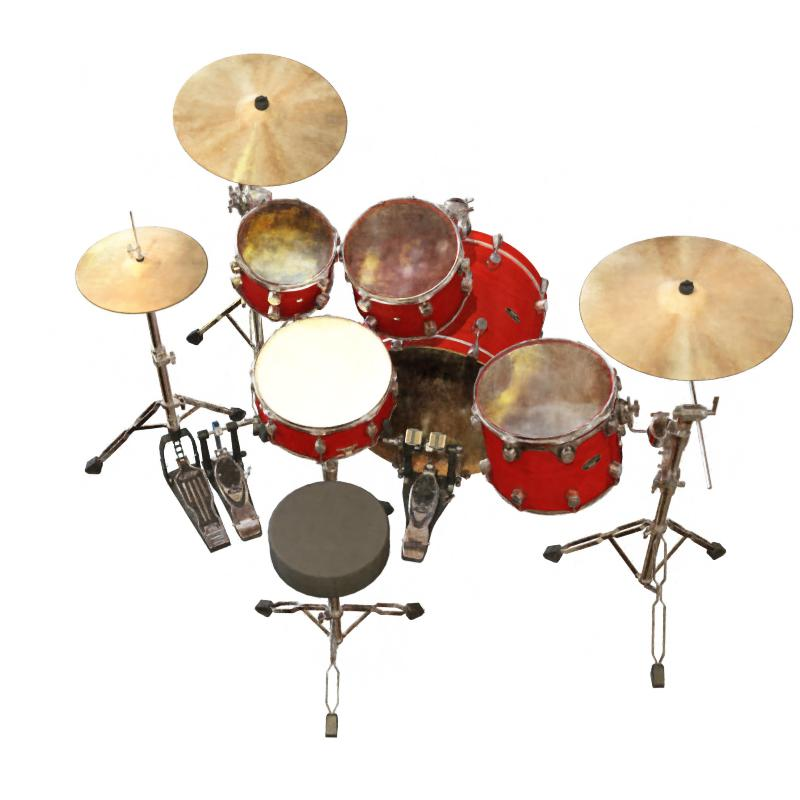
\includegraphics[scale=0.25]{img/mipnerf/mipnerf_drums_3.jpg}
			\caption{mip-NeRF}
		\end{subfigure}
		\begin{subfigure}{0.475\textwidth}
			\centering
			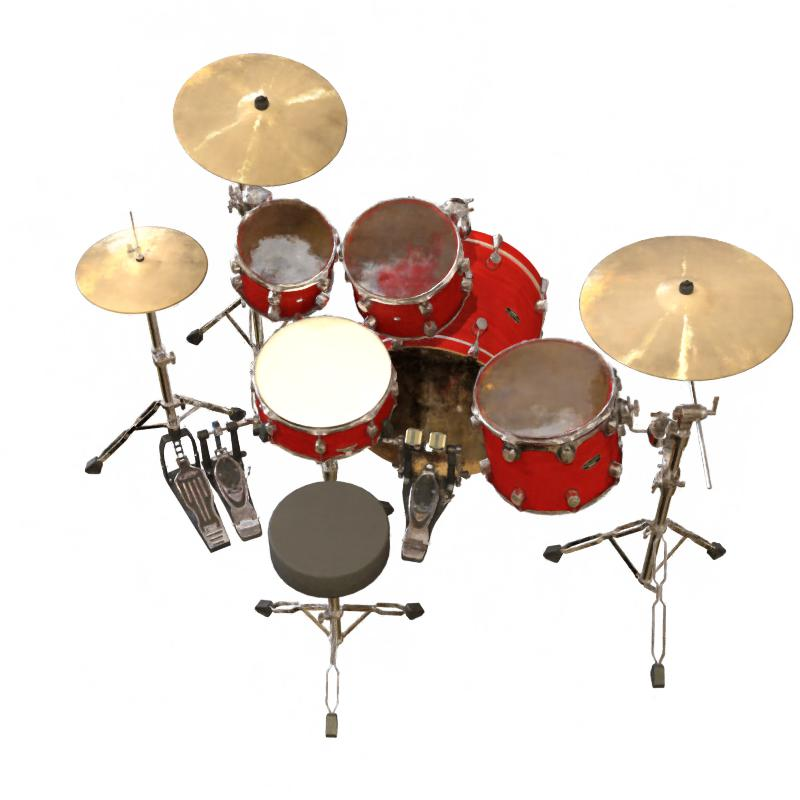
\includegraphics[scale=0.25]{img/refnerf/refnerf_drums_3.jpg}
			\caption{Ref-NeRF}
		\end{subfigure}
		\caption{Приказ резултата \textsc{Drums} скупа података}
		\label{fig-drums-results}
	\end{figure}

	\begin{figure}[H]
		\centering
		\begin{subfigure}{0.475\textwidth}
			\centering
			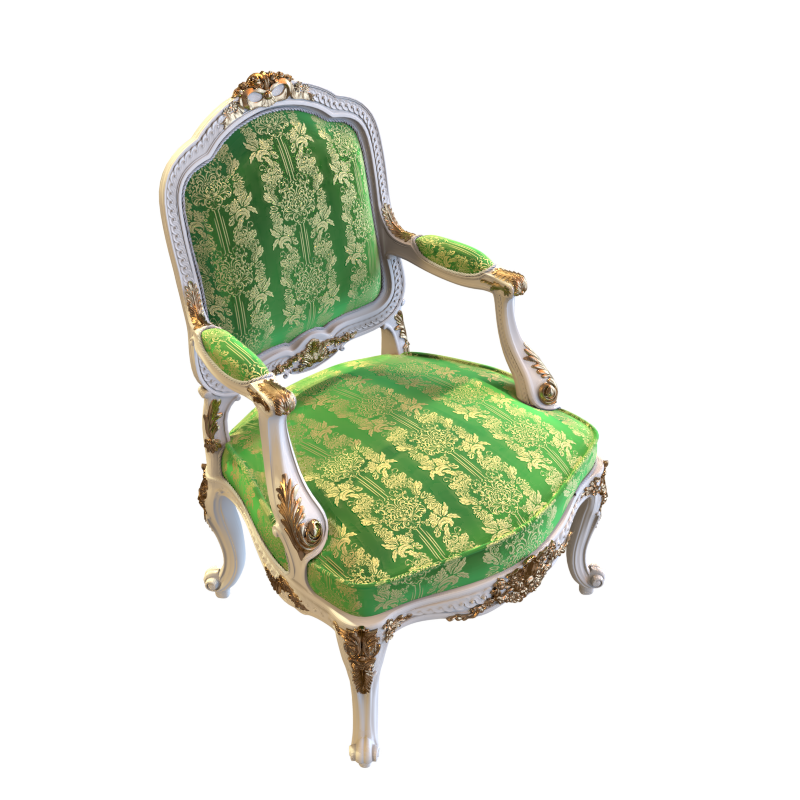
\includegraphics[scale=0.25]{img/gt/gt_chair_38.png}
			\caption{GT}
		\end{subfigure}
		\begin{subfigure}{0.475\textwidth}
			\centering
			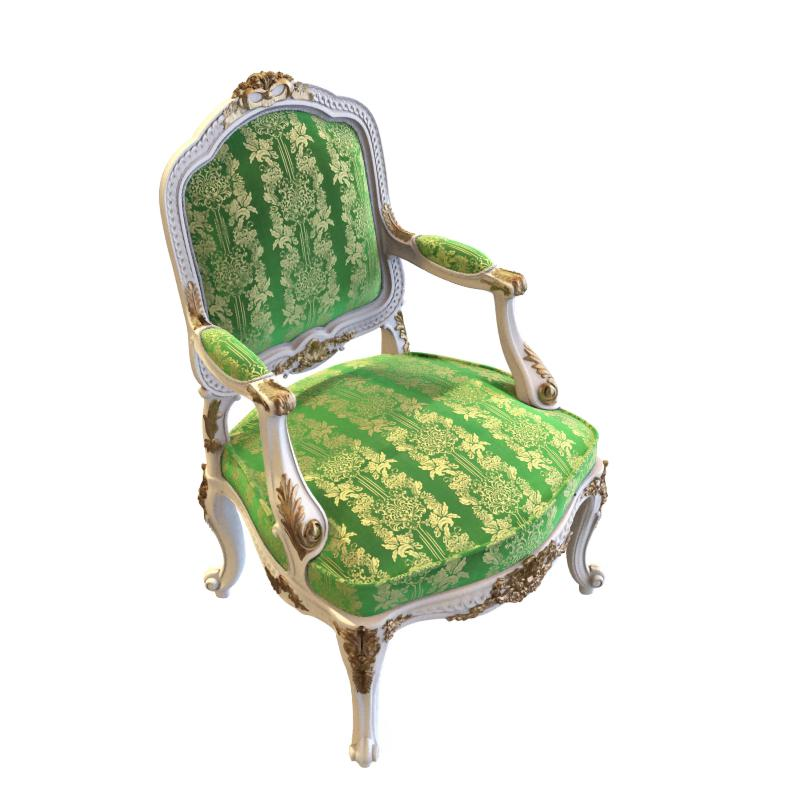
\includegraphics[scale=0.25]{img/nerf/nerf_chair_38.jpg}
			\caption{NeRF}
		\end{subfigure}
		\begin{subfigure}{0.475\textwidth}
			\centering
			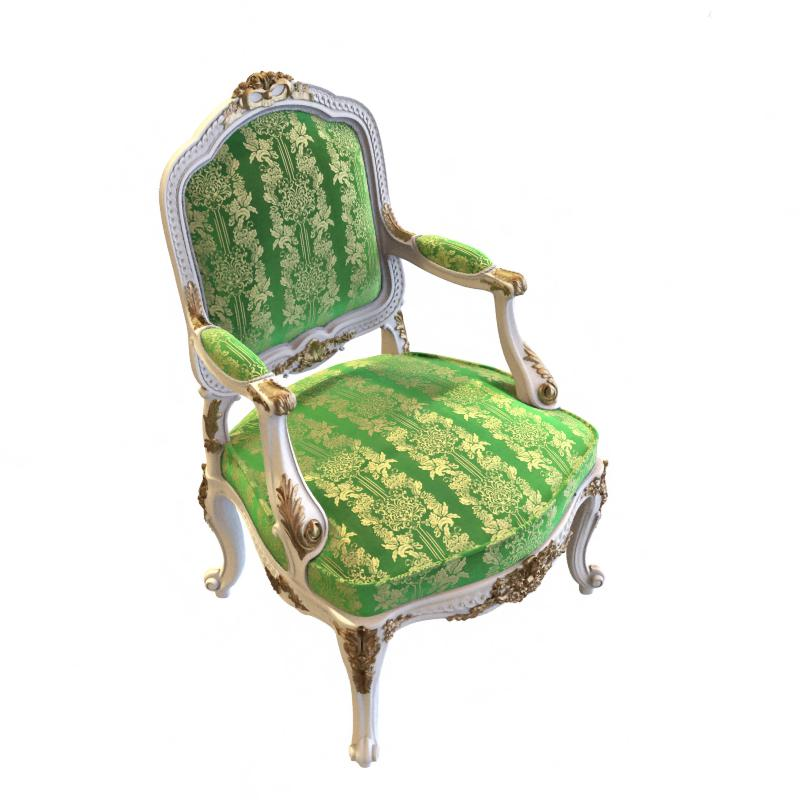
\includegraphics[scale=0.25]{img/mipnerf/mipnerf_chair_38.jpg}
			\caption{mip-NeRF}
		\end{subfigure}
		\begin{subfigure}{0.475\textwidth}
			\centering
			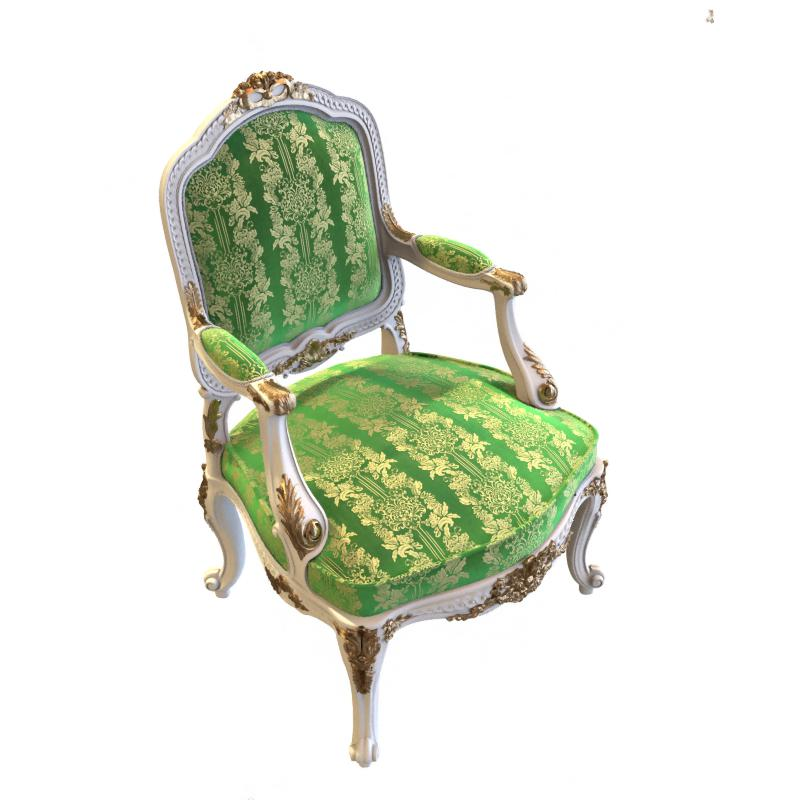
\includegraphics[scale=0.25]{img/refnerf/refnerf_chair_38.jpg}
			\caption{Ref-NeRF}
		\end{subfigure}
		\caption{Приказ резултата \textsc{Chair} скупа података}
		\label{fig-chair-results}
	\end{figure}

	\begin{figure}[H]
		\centering
		\begin{subfigure}{0.475\textwidth}
			\centering
			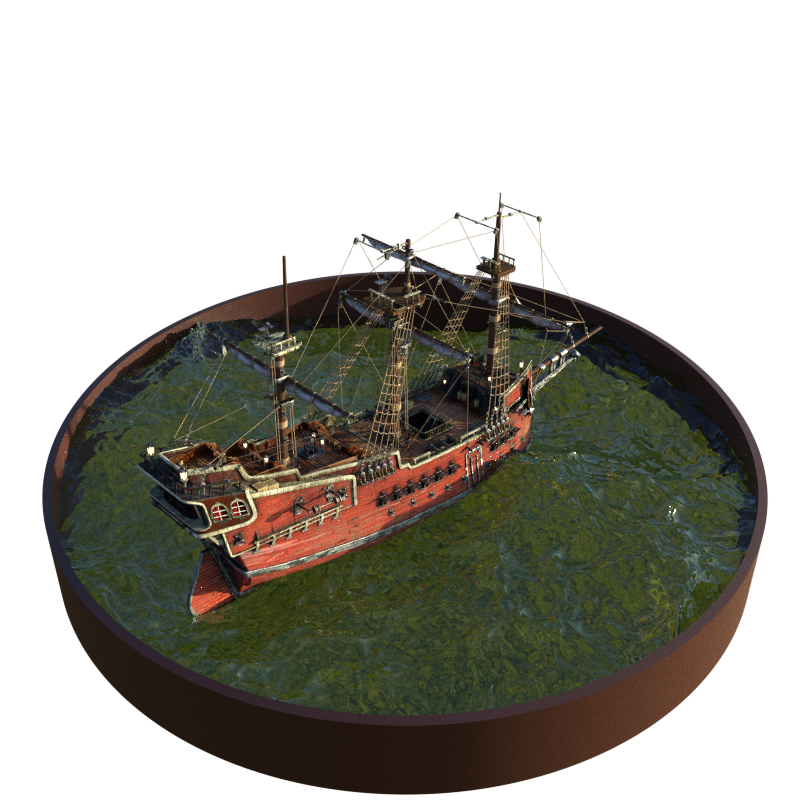
\includegraphics[scale=0.25]{img/gt/gt_ship_38.png}
			\caption{GT}
		\end{subfigure}
		\begin{subfigure}{0.475\textwidth}
			\centering
			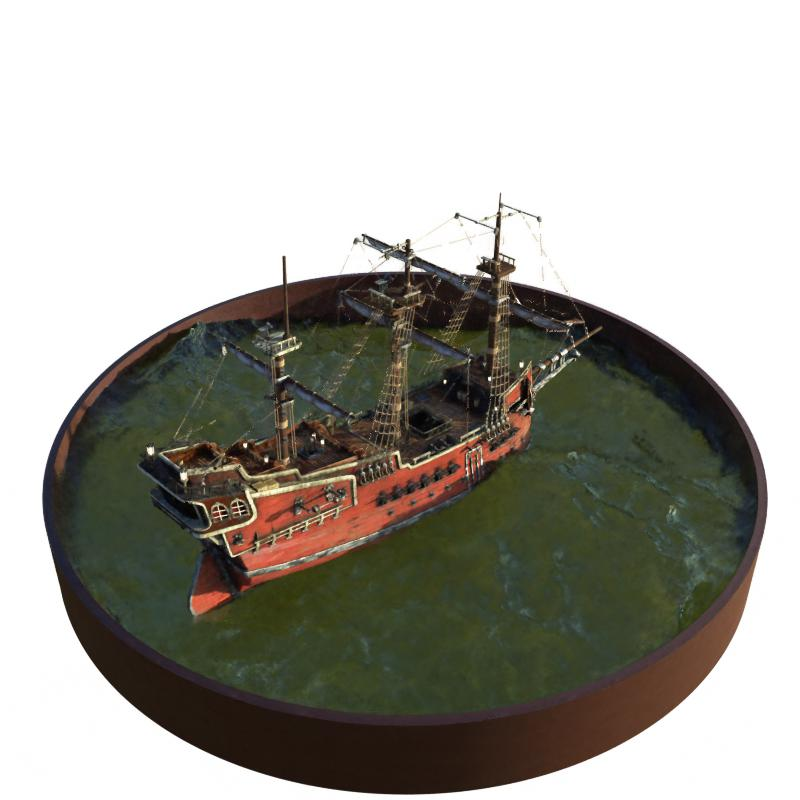
\includegraphics[scale=0.25]{img/nerf/nerf_ship_38.jpg}
			\caption{NeRF}
		\end{subfigure}
		\begin{subfigure}{0.475\textwidth}
			\centering
			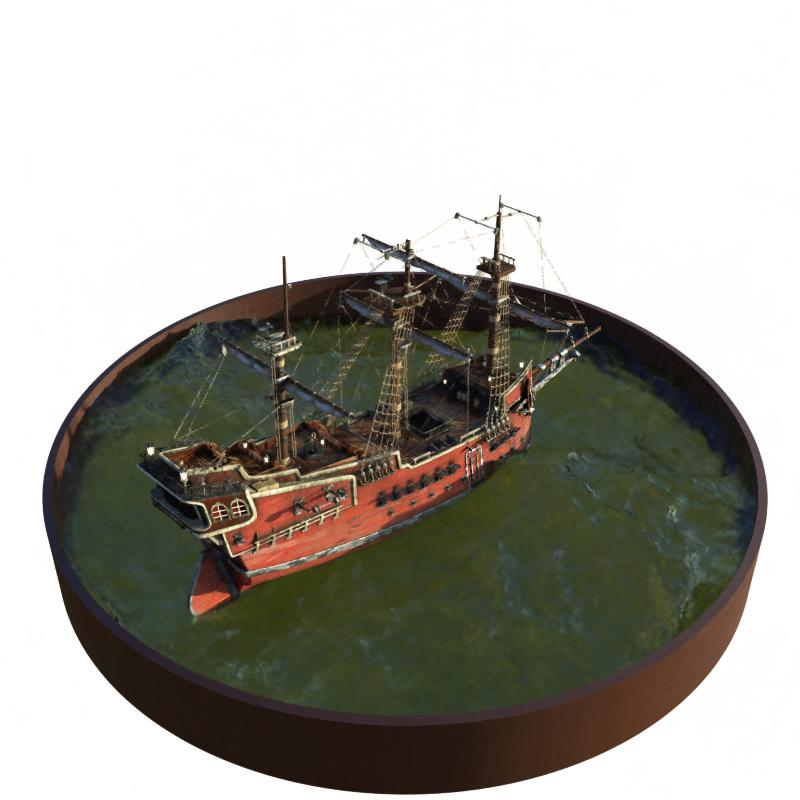
\includegraphics[scale=0.25]{img/mipnerf/mipnerf_ship_38.jpg}
			\caption{mip-NeRF}
		\end{subfigure}
		\begin{subfigure}{0.475\textwidth}
			\centering
			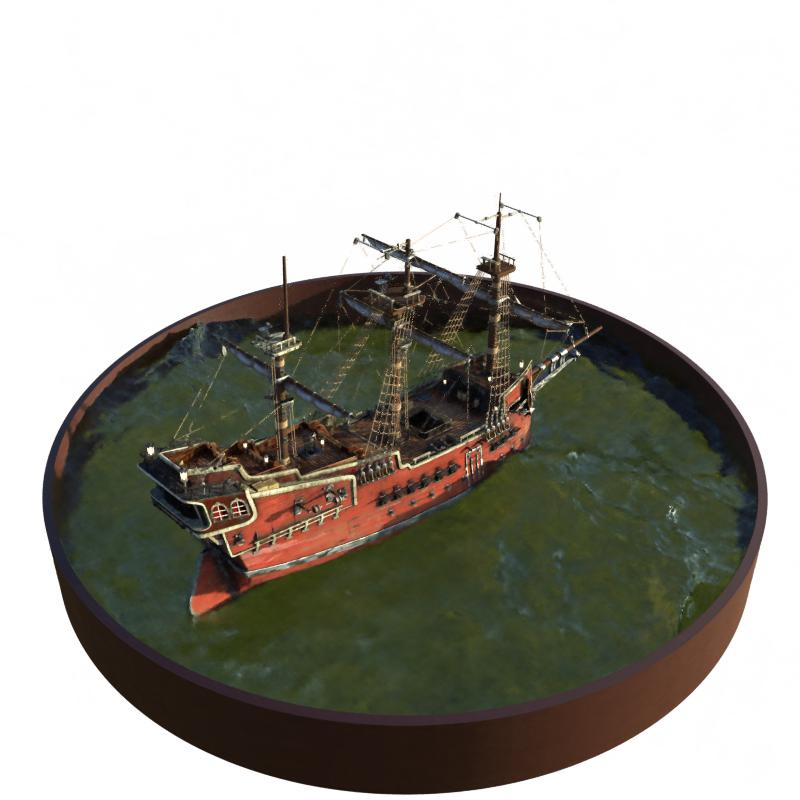
\includegraphics[scale=0.25]{img/refnerf/refnerf_ship_38.jpg}
			\caption{Ref-NeRF}
		\end{subfigure}
		\caption{Приказ резултата \textsc{Ship} скупа података}
		\label{fig-ship-results}
	\end{figure}

\section{Детаљно поређење}
Само гледањем резултата у претходној глави се поставља значајно питање -- постоје ли очите разлике у квалитету?
На основу метрика можемо видети да нема разлике у реду величине квалитета, али да очито постоје оне суптилније.
Зато ћемо се позабавити појединачним поређењем парова модела, а примере у којима то није изражено нећемо ни наводити.

\subsection{NeRF и mip-NeRF}
\subsection{NeRF и Ref-NeRF}
\subsection{mip-NeRF и Ref-NeRF}

\chapter{Закључак}
У овом раду су неуронска поља зрачења у потпуности теоријски заснована. Објашњени су основни физички и математички
концепти, уз одговарајућа образложења и разлоге увођења. Сви модели су успешно имплементирани, а искоришћен је и
пун потенцијал решења у облаку када је реч о њиховом обучавању. Резултати су приказани, а модели упоређени.
Можемо рећи да су постигнути резултати у складу са ауторским радовима.

Можемо рећи да је Ref-NeRF oднео победу и да се намеће као први избор. Иако је за обучавање овог модела потребно 
највише времена, у питању је разлика од највише 10\%. Побољшања су више него приметна без готово икаквих погоршања.
Преостала два модела нису \textit{значајно} лошија, тако да и њихово коришћење може дати задовољавајуће резултате.

Даљи рад се може сагледати на основу недостатака које су обрађени модели недвосмислено показали.
\begin{itemize}
	\item Неопходна је огромна рачунарска моћ. Обучавање траје дуго, а резултати још увек нису
	бољи, па чак ни једнаки, у поређењу са традиционалним приступима.
	\item Нити један од обрађених модела не може да ради у реалном времену.
	\item Неопходно је имати веома прецизну поставку сцене, а добијени модел jе обучен за само једну сцену.
\end{itemize}

На основу свега досад изреченог, можемо закључити да неуронска поља зрачења имају светлу будућност како у погледу
истраживања, тако и у погледу примене. У питању је млада област која има велики потенцијал.

\bibliographystyle{ieeetr}
\bibliography{refs}
\end{document}
